\documentclass[runningheads]{llncs}

% ---------------------------------------------------------------
% ECCV package must load first (provides xcolor, url, etc.)
\usepackage[review,year=2026,ID=5364]{eccv}

% ---------------------------------------------------------------
% Other packages
\usepackage{eccvabbrv}
\usepackage{graphicx}
\usepackage{booktabs}
\usepackage{amsmath,amssymb}
\usepackage{multirow}
\usepackage{listings}
\usepackage{algorithm}
\usepackage{algorithmic}
\usepackage{float}       % for [H] float placement
\usepackage{placeins}    % for \FloatBarrier
\usepackage[accsupp]{axessibility}
\usepackage[pagebackref,breaklinks,colorlinks,citecolor=eccvblue]{hyperref}
\usepackage[capitalize]{cleveref}
\usepackage{orcidlink}

% Listing style for prompt templates
\lstset{
  basicstyle=\ttfamily\footnotesize,
  breaklines=true,
  frame=single,
  backgroundcolor=\color{gray!5},
  rulecolor=\color{gray!40},
  xleftmargin=4pt,
  xrightmargin=4pt,
  aboveskip=6pt,
  belowskip=6pt,
}

\begin{document}

\title{UrbanAlign: Supplementary Material}
\titlerunning{UrbanAlign --- Supplementary}
\author{Anonymous ECCV 2026 Submission}
\authorrunning{Anonymous}
\institute{Anonymous Institution}
\maketitle

This supplementary document provides additional details that support the main paper.
\Cref{sec:dataset} describes the dataset filtering protocol and data-split statistics.
\Cref{sec:lwrr_weights} presents per-pair LWRR weight variation analysis.
\Cref{sec:sensitivity_full} reports full parameter-sweep grids expanding on the main-text sensitivity analysis.
\Cref{sec:prompts} reproduces the exact prompt templates used for multi-agent feature distillation.
\Cref{sec:theory} establishes the theoretical foundations: calibration bounds, local vs.\ global analysis, multi-agent variance reduction, and hybrid-space complementarity.
\Cref{sec:e2e} details the end-to-end dimension optimization procedure with trial-by-trial results across all six categories and a full API cost breakdown.
\Cref{sec:vrm_gain} reports per-mode LWRR alignment gains on \emph{wealthy}.
\Cref{sec:algorithm} provides the complete algorithm pseudocode.
\Cref{sec:preference_datasets} surveys related human preference datasets for potential transfer.
\Cref{sec:discussion} contains the full discussion: why post-hoc calibration works, local vs.\ global fitting, information-bottleneck connection, scope, limitations, ethics, and computational cost.
\textcolor{red}{\Cref{sec:backbone} reports open-source backbone generalization results with Qwen2.5-VL-72B.
\Cref{sec:reliability} provides bootstrap confidence intervals and human inter-annotator agreement analysis.}


% ==================================================================
% A. Dataset & Filtering Protocol
% ==================================================================
\section{Dataset and Filtering Protocol}
\label{sec:dataset}

\subsection{Place Pulse 2.0 Overview}

Place Pulse~2.0~\cite{salesses2013collaborative} contains 1,169,078 pairwise comparisons over 110,688 Google Street View images from 56 cities worldwide.
Each comparison asks: ``Which place looks more \texttt{<category>}?'' for six perception categories: \emph{safety}, \emph{lively}, \emph{beautiful}, \emph{wealthy}, \emph{depressing}, and \emph{boring}.
Each comparison yields one of three outcomes: \emph{left}, \emph{right}, or \emph{equal}.

\subsection{Consensus Filtering ($N \geq 2$)}

Raw Place Pulse data contains many image pairs with only a single vote, which carries high individual noise.
We apply a consensus threshold: only pairs with $N \geq 2$ independent votes and a strict majority ($> 50\%$ agreement on the winning label) are retained.
\Cref{tab:consensus} reports the full filtering statistics across all six categories.

\begin{table}[H]
\centering
\caption{Dataset filtering pipeline across all six perception categories. Raw pairs are unique image comparisons in Place Pulse~2.0. $N{\geq}2$ retains only pairs with at least two independent votes. Consensus (\%) is the average majority-vote agreement among retained pairs. All retained pairs are used in the experiments. Label distribution is by majority vote.}
\label{tab:consensus}
\small
\setlength{\tabcolsep}{3.5pt}
\begin{tabular}{lrrrrrr}
\toprule
Category & Raw Pairs & $N{\geq}2$ & Cons.\ (\%) & Left & Right & Equal \\
\midrule
Safety      & 360,095 & 1,412 & 87.6 & 682 & 652 & 78 \\
Beautiful   & 171,858 &   618 & 90.0 & 325 & 266 & 27 \\
Lively      & 260,428 & 1,288 & 85.8 & 595 & 613 & 80 \\
Wealthy     & 148,739 &   581 & 90.9 & 264 & 274 & 43 \\
Boring      & 124,371 &   449 & 90.3 & 211 & 206 & 32 \\
Depressing  & 129,229 &   471 & 91.4 & 223 & 230 & 18 \\
\midrule
\textbf{Total} & \textbf{1,194,720} & \textbf{4,819} & 89.3 & 2,300 & 2,241 & 278 \\
\bottomrule
\end{tabular}
\end{table}

\subsection{TrueSkill Rating Computation}

We convert the filtered pairwise votes into continuous per-image ratings using TrueSkill~\cite{herbrich2006trueskill} with priors
($\mu_0{=}25$, $\sigma_0{=}8.33$, $\beta{=}4.17$, draw prob.\ $=0.10$).
After convergence, images are ranked by $\mu$; the resulting values serve two purposes:
(1)~\emph{Stage~1 consensus sampling}: selecting high-$\mu$ and low-$\mu$ exemplars for dimension extraction;
(2)~\emph{Stage~3 supervision}: providing continuous TrueSkill score differences $y^{\mathrm{TS}}_{ij} {=} \mu_i {-} \mu_j$ as regression targets for LWRR.

\subsection{Data Split Protocol}

All retained pairs (449--1,412 per category) are partitioned into three disjoint sets:
\begin{itemize}
    \item \textbf{Reference set} $\mathcal{D}_{\mathrm{ref}}$ (60\%): provides human labels and TrueSkill supervision for LWRR calibration.
    Mirror augmentation doubles the effective reference size.
    \item \textbf{Validation set} $\mathcal{D}_{\mathrm{val}}$ (20\%): used for dimension search (Eq.~(2) in the main text) and hyperparameter selection ($N{=}50{,}000$ combined random search).
    \item \textbf{Test set} $\mathcal{D}_{\mathrm{test}}$ (20\%): held out for final evaluation; never used for any tuning decision.
\end{itemize}
The split uses a fixed random seed (42) for reproducibility.
$\mathcal{D}_{\mathrm{ref}} \cap \mathcal{D}_{\mathrm{val}} \cap \mathcal{D}_{\mathrm{test}} = \varnothing$ by construction.
After excluding human ``equal'' labels, 83--260 test pairs per category remain.

\subsection{Dataset Distribution}

\Cref{fig:pairs_dist} shows the distribution of image pairs across vote thresholds for all six categories.
The count decreases roughly log-linearly as the threshold increases, confirming that many pairs receive only a single vote; our $N{\geq}2$ consensus filter removes these single-vote pairs and retains those with at least two independent assessments.
\Cref{fig:images_dist} shows the individual image appearance frequency: most images appear in fewer than 5 comparisons, while a heavy tail of frequently compared images provides stable TrueSkill estimates.

\begin{figure}[H]
\centering
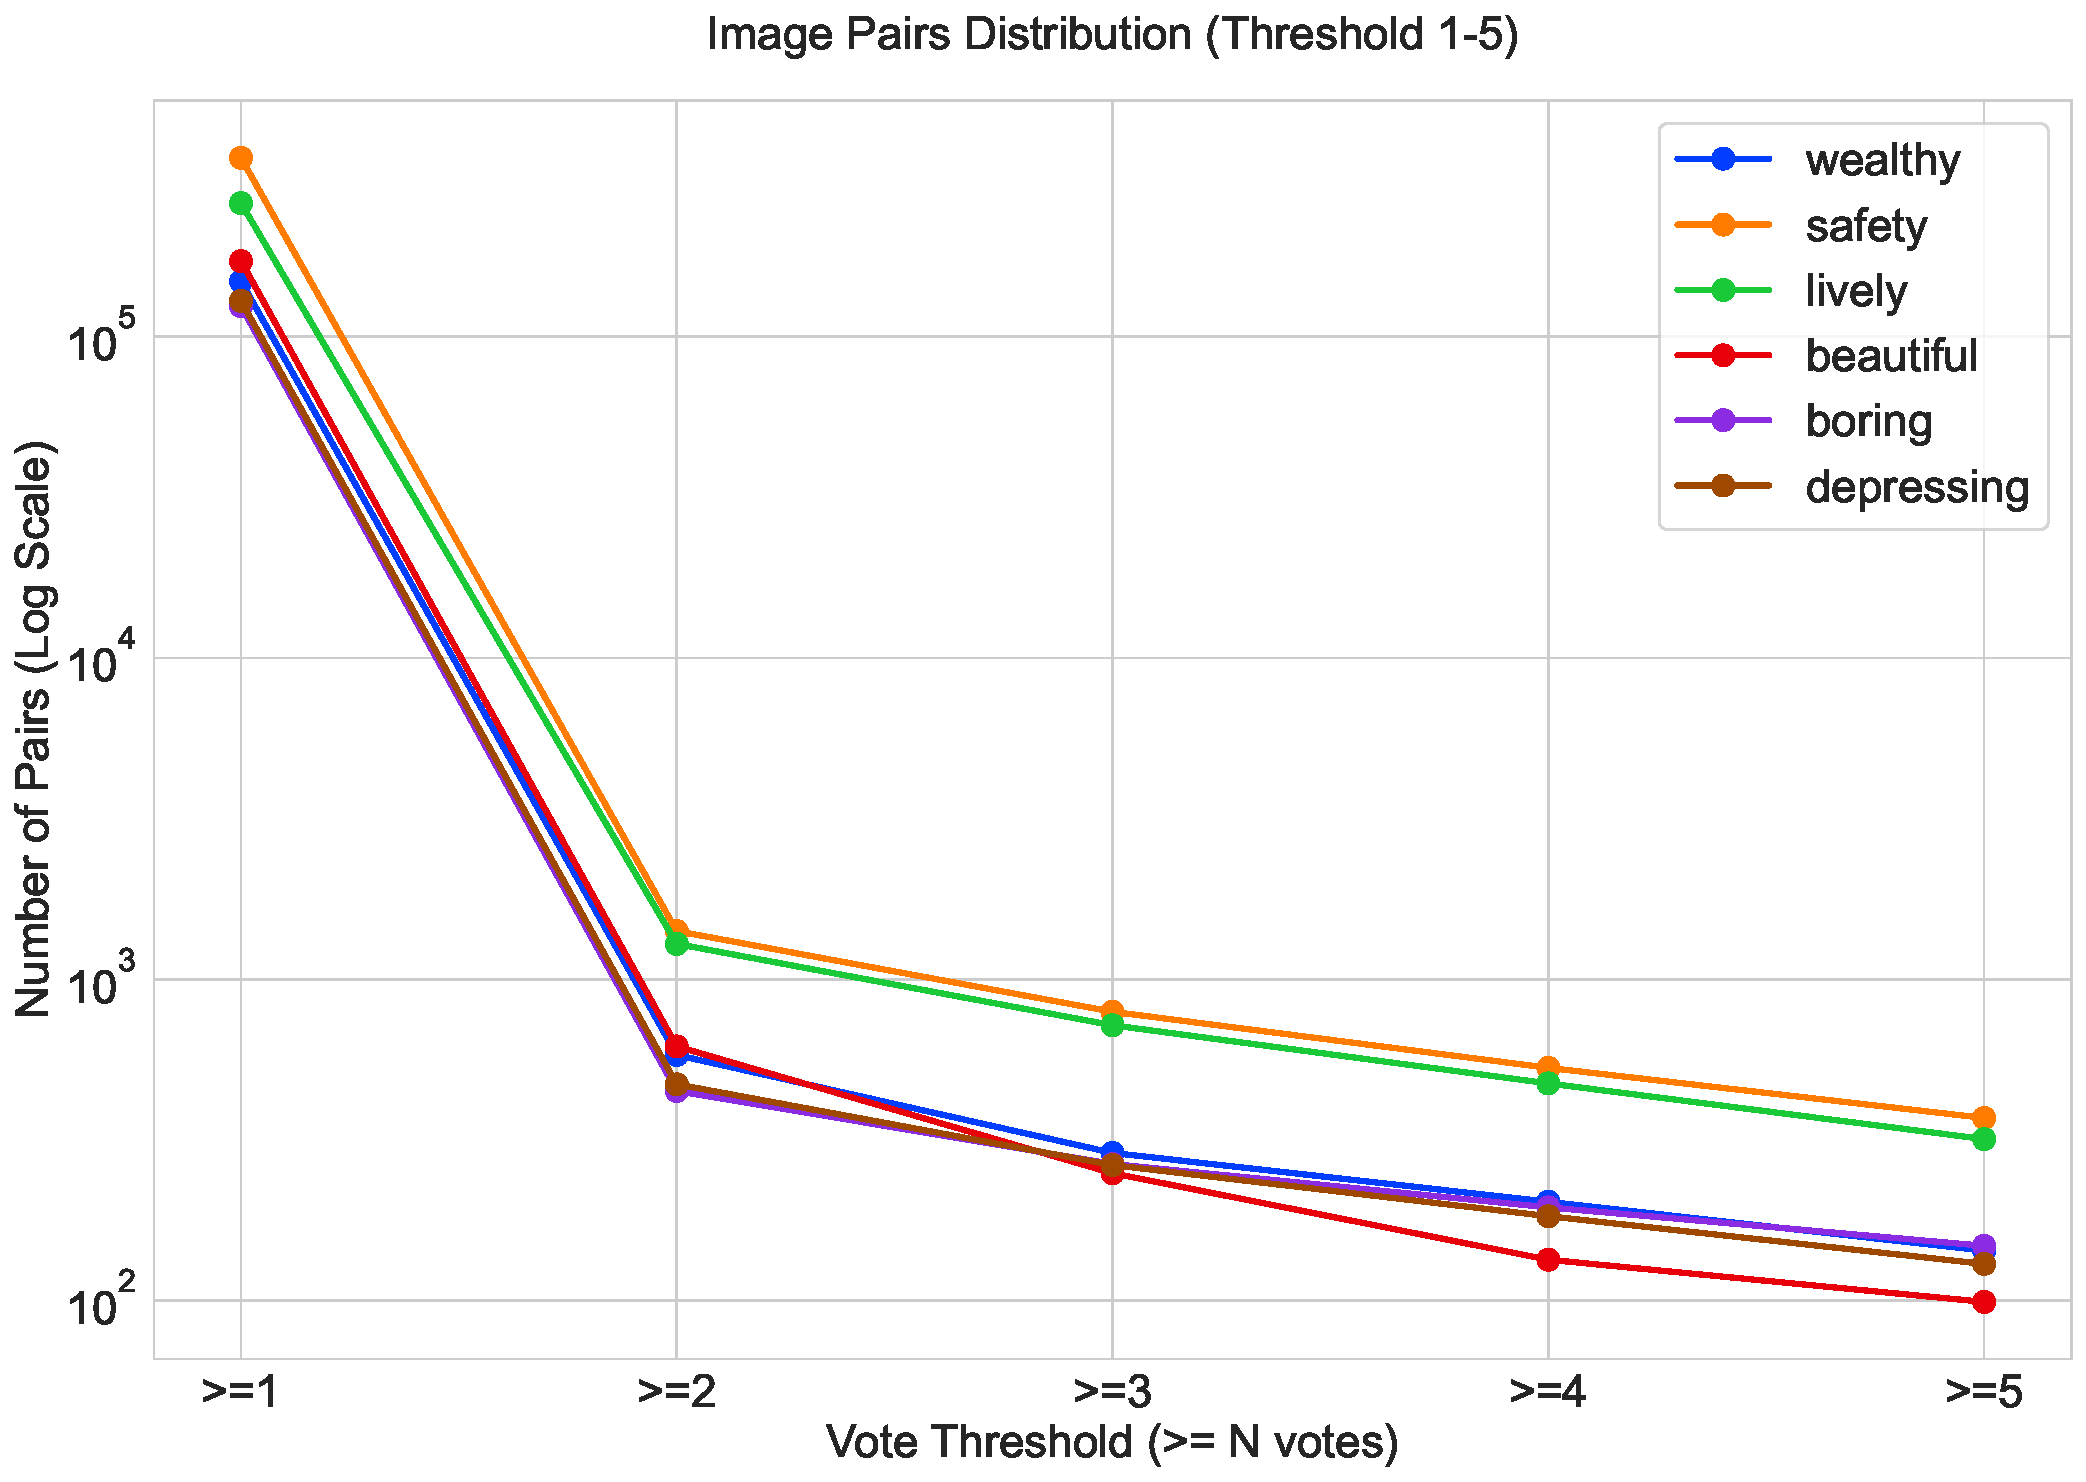
\includegraphics[width=0.85\textwidth]{human_pairs_distribution.pdf}
\caption{Distribution of image pairs across vote thresholds (${\geq}1$ to ${\geq}5$ votes) for all six perception categories. The $y$-axis is log-scaled. Our consensus filter retains pairs with $N{\geq}2$ votes.}
\label{fig:pairs_dist}
\end{figure}

\begin{figure}[H]
\centering
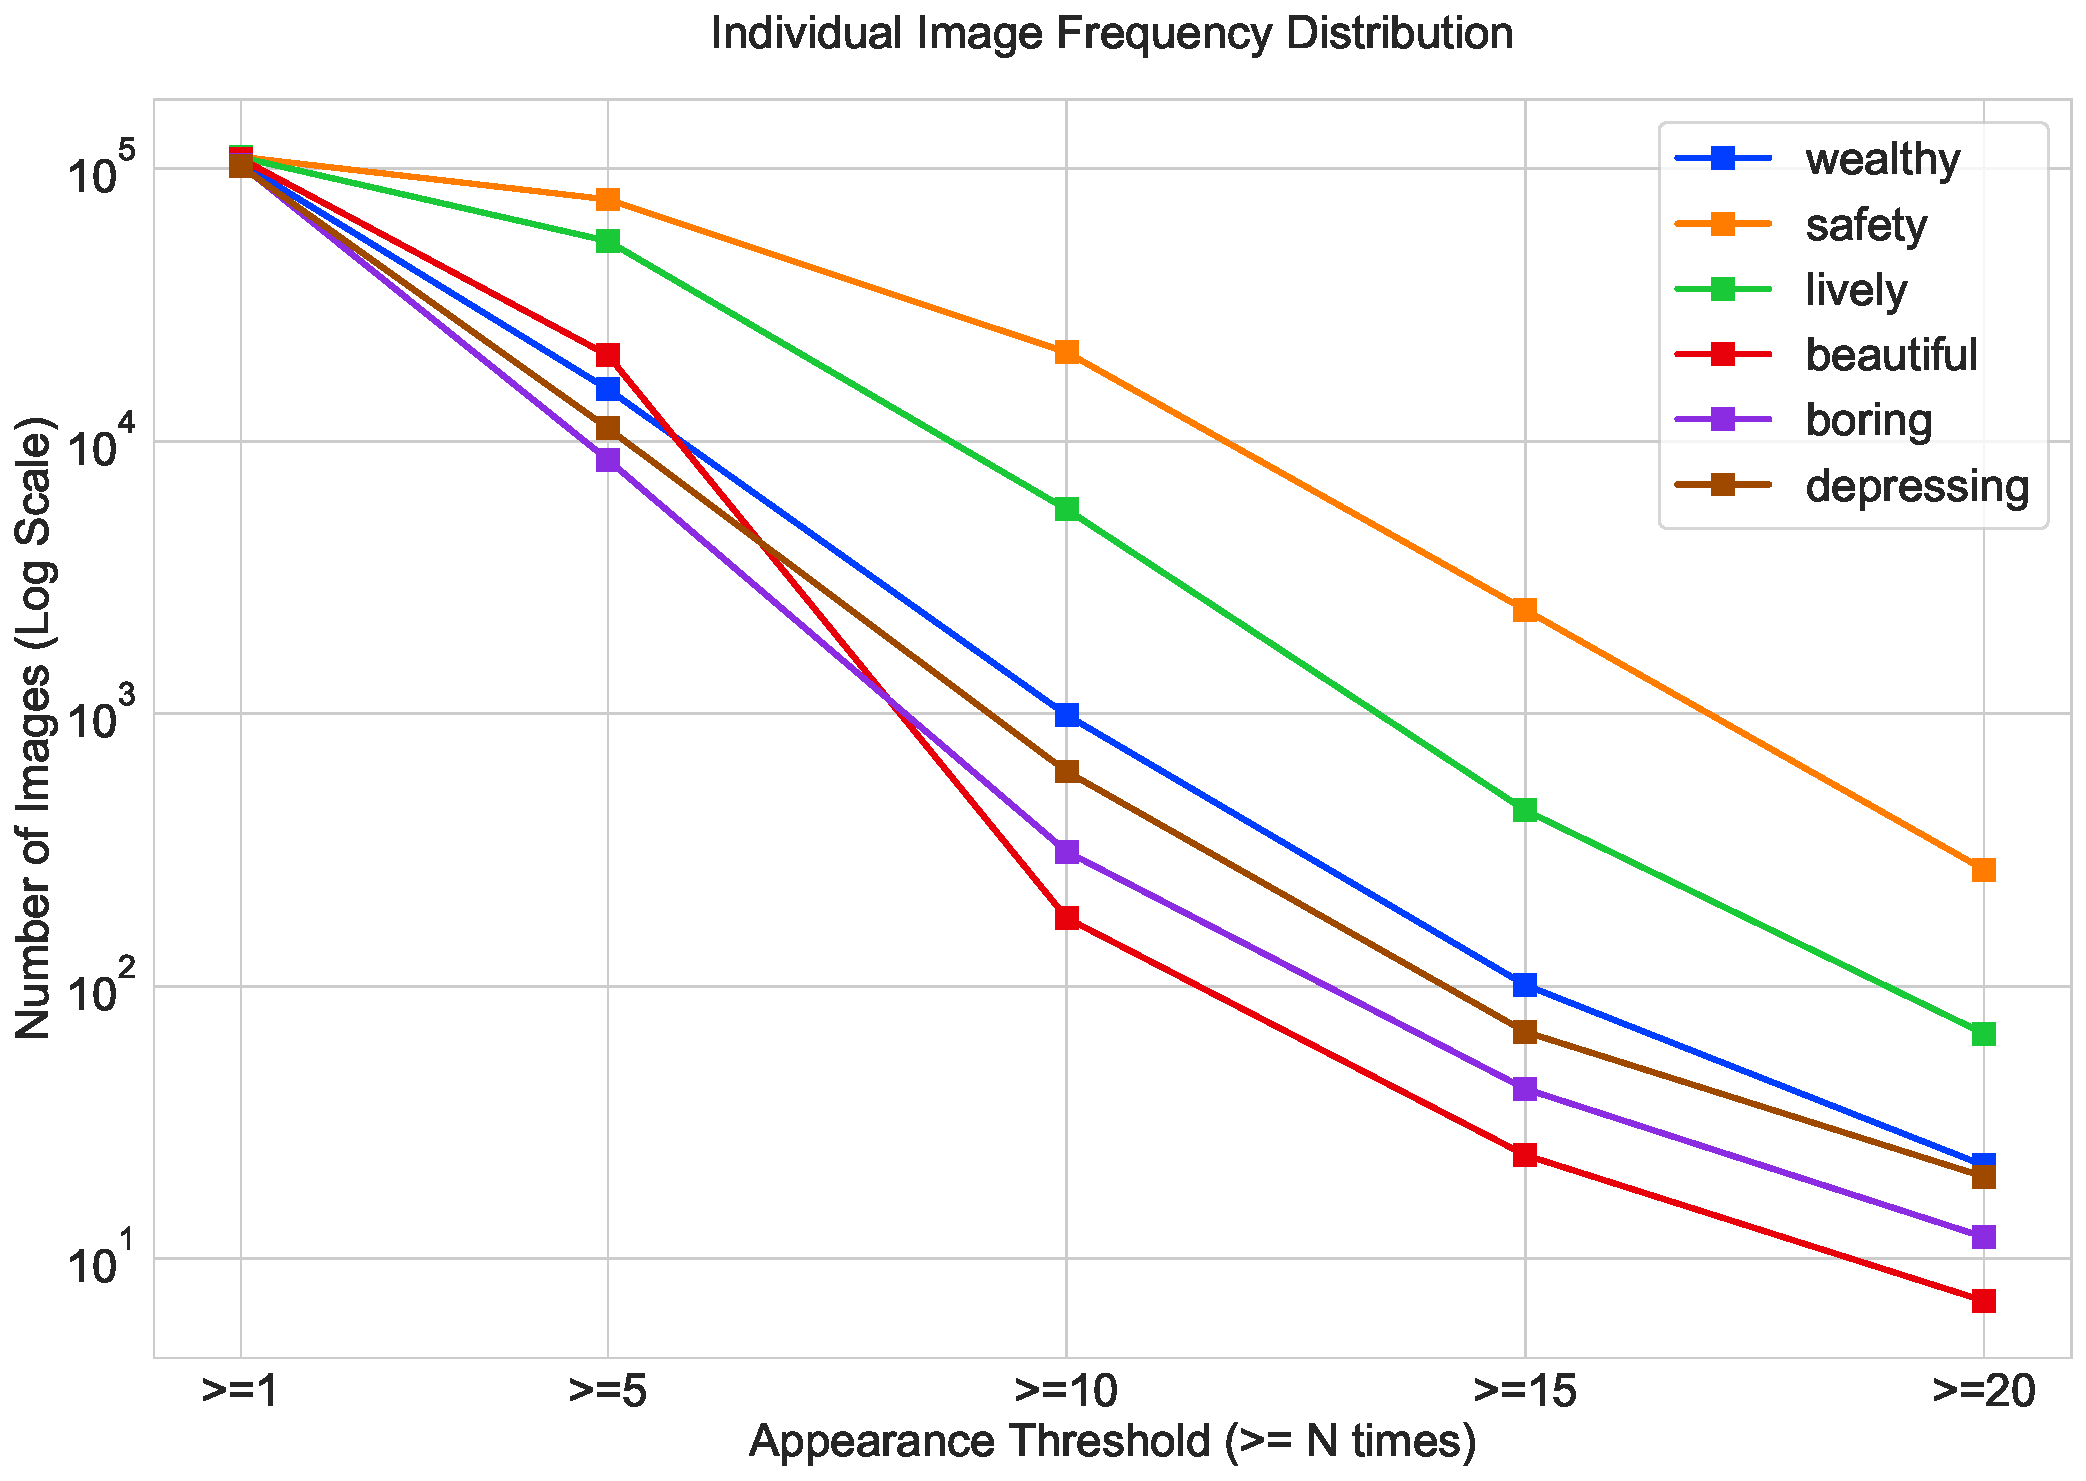
\includegraphics[width=0.85\textwidth]{human_images_distribution.pdf}
\caption{Individual image appearance frequency distribution across thresholds (${\geq}1$ to ${\geq}20$ appearances) for all six categories. The heavy-tailed distribution indicates a core set of frequently compared images that anchor TrueSkill rating estimates.}
\label{fig:images_dist}
\end{figure}


% ==================================================================
% B. LWRR Per-Pair Weight Analysis
% ==================================================================
\section{LWRR Per-Pair Weight Analysis}
\label{sec:lwrr_weights}

A key feature of LWRR is that each test pair receives its \emph{own} locally-fitted weight vector $\hat{\mathbf{w}} \in \mathbb{R}^{n}$ ($n{=}8$ for \emph{wealthy}), reflecting the dimension importances in its particular neighbourhood of the hybrid manifold.
This contrasts with a global linear model where all pairs share the same weights.

\subsection{Weight Variation Across the Manifold}

\Cref{tab:weight_variation} reports the mean and standard deviation of each dimension's local weight across all 117 test pairs.
High standard deviation indicates that the dimension's importance varies substantially across different regions of the perception manifold---precisely the heterogeneity that motivates local rather than global calibration.

\begin{table}[H]
\centering
\caption{LWRR local weight statistics across 117 test pairs (\emph{wealthy} category, Mode~4).}
\label{tab:weight_variation}
\small
\begin{tabular}{lccc}
\toprule
Dimension & Mean $w$ & Std $w$ & CV \\
\midrule
Building Modernity        & 2.305 & 2.676 & 1.16 \\
Infrastructure Condition  & $-$1.858 & 2.074 & 1.12 \\
Vegetation Maintenance    & 1.722 & 1.996 & 1.16 \\
Street Cleanliness        & 1.355 & 1.318 & 0.97 \\
Pavement Integrity        & $-$1.068 & 2.387 & 2.23 \\
Vehicle Quality           & $-$1.043 & 1.763 & 1.69 \\
Fa\c{c}ade Quality       & $-$0.921 & 1.663 & 1.81 \\
Lighting Quality          & 0.241 & 1.464 & 6.08 \\
\bottomrule
\end{tabular}
\\[4pt]
\footnotesize{CV = Coefficient of Variation ($\mathrm{Std}/|\mathrm{Mean}|$). Higher CV indicates greater spatial heterogeneity of dimension importance. Sorted by $|\text{Mean}|$.}
\end{table}

\Cref{tab:weight_variation_all} extends this analysis to all six categories.

\begin{table}[H]
\centering
\caption{Top-3 LWRR local weights by $|\text{Mean}|$ for each perception category (Mode~4). High Std relative to Mean confirms that dimension importance varies substantially across the manifold.}
\label{tab:weight_variation_all}
\small
\setlength{\tabcolsep}{4pt}
\begin{tabular}{llccc}
\toprule
Category & Dimension & Mean $w$ & Std $w$ & CV \\
\midrule
\multirow{3}{*}{Safety ($n{=}283$)}
& Visibility Clarity      & $-$0.421 & 1.702 & 4.04 \\
& Lighting Adequacy        & 0.291  & 1.401 & 4.81 \\
& Building Maintenance     & 0.280  & 1.311 & 4.67 \\
\midrule
\multirow{3}{*}{Beautiful ($n{=}125$)}
& Arch.\ Coherence         & 1.471  & 4.825 & 3.28 \\
& Visual Complexity        & 1.193  & 10.960 & 9.19 \\
& Pedestrian Amenities     & 0.887  & 4.901 & 5.53 \\
\midrule
\multirow{3}{*}{Lively ($n{=}259$)}
& Commercial Activity      & $-$0.518 & 0.413 & 0.80 \\
& Color \& Lighting        & 0.263  & 0.404 & 1.53 \\
& Street Furniture         & 0.115  & 0.296 & 2.58 \\
\midrule
\multirow{3}{*}{Wealthy ($n{=}117$)}
& Building Modernity       & 2.305  & 2.676 & 1.16 \\
& Infrastructure Cond.     & $-$1.858 & 2.074 & 1.12 \\
& Vegetation Maint.        & 1.722  & 1.996 & 1.16 \\
\midrule
\multirow{3}{*}{Boring ($n{=}91$)}
& Color Vibrancy           & $-$1.068 & 1.680 & 1.57 \\
& Visual Complexity        & 0.531  & 1.438 & 2.71 \\
& Arch.\ Diversity         & 0.347  & 1.103 & 3.18 \\
\midrule
\multirow{3}{*}{Depressing ($n{=}95$)}
& Greenery Presence        & 0.649  & 1.260 & 1.94 \\
& Lighting Quality         & $-$0.503 & 1.555 & 3.09 \\
& Fa\c{c}ade Condition     & 0.213  & 1.329 & 6.24 \\
\bottomrule
\end{tabular}
\end{table}

\subsection{Illustrative Examples}

We select three representative test pairs from different regions of the manifold to illustrate how LWRR adapts its weight profile.

\medskip\noindent\textbf{Example 1: Vegetation-driven pair.}
In the suburban portion of the manifold, LWRR assigns dominant weights to Vegetation Maintenance ($w{=}3.38$) and Building Modernity ($w{=}1.17$), while Fa\c{c}ade Quality receives near-zero weight ($w{\approx}-0.94$).
This reflects the perceptual pattern that in residential areas, landscaping quality is the primary cue for perceived wealth.

\medskip\noindent\textbf{Example 2: Infrastructure-driven pair.}
In the dense urban core, the local weight profile shifts: Infrastructure Condition ($w{=}1.01$) and Vehicle Quality ($w{=}-1.18$) dominate, while Vegetation drops.
The sign reversal on Vehicle Quality indicates contextual inversion---in downtown areas, the presence of high-end vehicles may signal commercial rather than residential wealth.

\medskip\noindent\textbf{Example 3: Balanced transitional pair.}
Pairs in mixed-use zones show relatively uniform weight magnitude across all seven dimensions (std of $|w|$ across dims $<$0.5), confirming that these regions lack a single dominant perceptual cue.
The high CV (Coefficient of Variation $>$3) for Lighting Quality (6.08) in \cref{tab:weight_variation} is driven precisely by these transitional pairs.

\medskip
These examples confirm the theoretical motivation for local calibration: the dimensions that matter most for perceiving ``wealth'' depend on the visual context.
A single global weight vector would average over these distinct regimes, losing the nuance that LWRR captures.


% ==================================================================
% C. Detailed Sensitivity Analysis
% ==================================================================
\section{Detailed Sensitivity Analysis}
\label{sec:sensitivity_full}

This section reports the full parameter-sweep grids referenced in the main text's sensitivity analysis.
Each experiment varies one parameter at a time while holding others at their defaults ($K{=}20$, $\alpha{=}0.3$, $\tau_{\mathrm{kernel}}{=}1.0$, $\lambda{=}1.0$, $\varepsilon{=}0.8$, $\theta{=}0.6$).
All results are Mode~4, accuracy excluding ``equal'' human labels.

\subsection{Neighbourhood Size $K_{\max}$}

\begin{table}[H]
\centering
\caption{Full $K_{\max}$ sweep (Mode~4, all categories, accuracy \% excl.\ equal).}
\label{tab:k_sweep}
\small
\setlength{\tabcolsep}{4pt}
\begin{tabular}{ccccccc|c}
\toprule
$K_{\max}$ & Safety & Beaut. & Lively & Wealthy & Boring & Depress. & Avg \\
\midrule
10 & 59.2 & 50.7 & 51.3 & 55.7 & 53.6 & 54.1 & 54.1 \\
20 & \textbf{66.7} & 53.8 & \textbf{61.3} & \textbf{57.1} & 52.8 & 58.6 & \textbf{58.4} \\
30 & 70.3 & 52.2 & 61.6 & 49.3 & 50.7 & 55.6 & 56.6 \\
50 & 66.7 & \textbf{54.4} & 55.6 & 52.6 & \textbf{58.6} & \textbf{57.4} & 57.6 \\
\bottomrule
\end{tabular}
\end{table}

\noindent\textbf{Analysis.}
Small $K$ ($=10$) leads to high-variance local fits (each ridge regression uses very few reference points).
$K{=}20$ achieves the best average (58.4\%). However, the optimal $K$ varies per category: \emph{safety} favours $K{=}30$ (70.3\%), while \emph{boring} favours $K{=}50$ (58.6\%), reflecting different local densities of the reference manifold across categories.

\subsection{Hybrid Weight $\alpha$}

\begin{table}[H]
\centering
\caption{Full $\alpha$ sweep (Mode~4, all categories, accuracy \% excl.\ equal).}
\label{tab:alpha_sweep}
\small
\setlength{\tabcolsep}{4pt}
\begin{tabular}{cccccccc|c}
\toprule
$\alpha$ & Sem.\ Wt. & Safety & Beaut. & Lively & Wealthy & Boring & Depress. & Avg \\
\midrule
0.1 & 90\% & 61.3 & 52.9 & 57.9 & 55.6 & 50.0 & 57.8 & 55.9 \\
0.2 & 80\% & 64.6 & 54.5 & 57.3 & 56.4 & 52.9 & 58.8 & 57.4 \\
0.3 & 70\% & \textbf{66.7} & 53.8 & \textbf{61.3} & \textbf{57.1} & 52.8 & 58.6 & \textbf{58.4} \\
0.5 & 50\% & 62.0 & 56.1 & 49.3 & 56.8 & 52.1 & 56.9 & 55.5 \\
0.7 & 30\% & 62.0 & \textbf{60.3} & 51.4 & 54.4 & \textbf{58.0} & \textbf{62.5} & 58.1 \\
\bottomrule
\end{tabular}
\end{table}

\noindent\textbf{Analysis.}
$\alpha{=}0.3$ (70\% semantic weight) is optimal on average, but per-category optima differ notably: \emph{beautiful} favours $\alpha{=}0.7$ (60.3\%) and \emph{depressing} also favours $\alpha{=}0.7$ (62.5\%), suggesting that CLIP features carry more discriminative signal for aesthetics-related categories.
Pure CLIP ($\alpha{=}1.0$) performs poorly because CLIP's pre-training distribution (web images of objects) is mismatched with street-view perception tasks.
This empirically validates our hybrid design while highlighting category-specific tuning opportunities.

\textcolor{red}{\smallskip\noindent\textbf{Hybrid vs.\ semantic-only under LWRR.}
A reviewer concern is that global ridge on hybrid features (57.8\%) underperforms semantic-only (61.2\%) in the main text, questioning whether CLIP helps.
The alpha sweep confirms that CLIP contributes via \emph{neighbourhood structure}, not global discriminability: LWRR at $\alpha{=}0.3$ (58.4\% avg) outperforms $\alpha{=}0.1$ (55.9\% avg, nearly semantic-only) by +2.5\,pp, with consistent gains on 5/6 categories (\emph{safety}: +5.4\,pp, \emph{lively}: +3.4\,pp).
The global ridge result (57.8\% hybrid $<$ 61.2\% semantic) reflects the \emph{global} model's inability to exploit CLIP's neighbourhood signal: adding CLIP features increases global regression dimensionality without local adaptation.
LWRR resolves this by using CLIP for neighbourhood selection while fitting only on semantic differentials, as formalised in \cref{prop:hybrid}.}

\subsection{Kernel Bandwidth $\tau_{\mathrm{kernel}}$}

\begin{table}[H]
\centering
\caption{Full $\tau_{\mathrm{kernel}}$ sweep (Mode~4, \emph{wealthy}).}
\label{tab:tau_sweep}
\small
\begin{tabular}{cccc}
\toprule
$\tau_{\mathrm{kernel}}$ & Acc (\%) & $\kappa$ & $N_{\mathrm{aligned}}$ \\
\midrule
0.1 & 54.9 & 0.09 & 87 \\
0.3 & 56.1 & 0.12 & 87 \\
0.5 & 56.8 & 0.13 & 87 \\
0.8 & 57.0 & 0.13 & 87 \\
1.0 & 57.1 & 0.13 & 87 \\
\bottomrule
\end{tabular}
\end{table}

\noindent\textbf{Analysis.}
Smaller $\tau$ concentrates weight on the nearest neighbours (sharper kernel); larger $\tau$ approaches uniform weighting within the $K$-neighbourhood.
The relatively flat response across the tested range ($<$2.2\,pp variation) suggests that the $K$-NN pre-selection already isolates relevant neighbours, making the exact kernel bandwidth less critical.

\subsection{Ridge Penalty $\lambda_{\mathrm{ridge}}$}

\begin{table}[H]
\centering
\caption{Full $\lambda_{\mathrm{ridge}}$ sweep (Mode~4, \emph{wealthy}).}
\label{tab:lambda_sweep}
\small
\begin{tabular}{cccc}
\toprule
$\lambda$ & Acc (\%) & $\kappa$ & $N_{\mathrm{aligned}}$ \\
\midrule
0.01 & 56.1 & 0.12 & 87 \\
0.05 & 56.1 & 0.12 & 87 \\
0.1  & 56.1 & 0.12 & 87 \\
0.5  & 56.8 & 0.13 & 87 \\
1.0  & 57.1 & 0.13 & 87 \\
\bottomrule
\end{tabular}
\end{table}

\noindent\textbf{Analysis.}
The ridge penalty $\lambda$ has minimal impact across several orders of magnitude ($<$1.0\,pp variation).
This is expected: with $K{=}20$ neighbours and $n{=}8$ dimensions, the system is well-overdetermined ($K \gg n$), so regularisation has little effect.

\subsection{Equal Threshold $\varepsilon$ (EQUAL\_EPS)}

\begin{table}[H]
\centering
\caption{Full $\varepsilon$ (EQUAL\_EPS) sweep (Mode~4, all categories, accuracy \% excl.\ equal).}
\label{tab:eps_sweep}
\small
\setlength{\tabcolsep}{4pt}
\begin{tabular}{ccccccc|c}
\toprule
$\varepsilon$ & Safety & Beaut. & Lively & Wealthy & Boring & Depress. & Avg \\
\midrule
0.3 & 65.0 & 52.2 & 60.3 & 57.3 & 52.1 & 56.9 & 57.3 \\
0.5 & 65.0 & 52.2 & 60.3 & 57.3 & 52.1 & 56.9 & 57.3 \\
0.8 & 66.7 & 53.8 & 61.3 & 57.1 & \textbf{52.8} & 58.6 & 58.4 \\
1.2 & 67.6 & 54.1 & 61.3 & 57.3 & 51.5 & 56.7 & 58.1 \\
2.0 & \textbf{67.1} & \textbf{50.9} & \textbf{60.3} & \textbf{57.5} & 49.2 & \textbf{54.8} & 56.6 \\
\bottomrule
\end{tabular}
\end{table}

\noindent\textbf{Analysis.}
The equal threshold $\varepsilon$ shows that the default value of $\varepsilon{=}0.8$ achieves the best average at 58.4\%, with moderate variation across the tested range ($<$1.8\,pp).
This suggests that many borderline pairs are better classified as non-equal, potentially because the VLM's score differences carry marginal but genuine signal even for close pairs.

\subsection{Combined Search}

In addition to the one-at-a-time sweeps above, we performed a random search over the combined parameter space ($N{=}50{,}000$ configurations) to check for interactions.
\Cref{tab:combined_sweep} reports the per-category best configurations found.

\begin{table}[H]
\centering
\caption{Best per-category configurations from combined random search (Mode~4, accuracy \% excl.\ equal).}
\label{tab:combined_sweep}
\small
\setlength{\tabcolsep}{4pt}
\begin{tabular}{lccl}
\toprule
Category & Acc.\ (\%) & $\kappa$ & Key Parameters \\
\midrule
Safety      & 81.6 & 0.636 & $K{=}30$, $\alpha{=}0.2$, sel${=}0.6$ \\
Beautiful   & 69.8 & 0.384 & $K{=}10$, $\alpha{=}0.5$, sel${=}0.6$ \\
Lively      & 69.4 & 0.404 & $K{=}50$, $\alpha{=}0.7$, sel${=}0.6$ \\
Wealthy     & 74.0 & 0.480 & $K{=}50$, $\alpha{=}0.7$, sel${=}0.6$ \\
Boring      & 70.2 & 0.414 & $K{=}30$, $\alpha{=}0.7$, sel${=}0.6$ \\
Depressing  & 68.2 & 0.370 & $K{=}20$, $\alpha{=}0.2$, sel${=}0.6$ \\
\midrule
Average     & 72.2 & 0.448 & --- \\
\bottomrule
\end{tabular}
\end{table}

\noindent The combined search yields 72.2\% average accuracy ($\kappa{=}0.448$), a +13.8\,pp gain over the default configuration (58.4\%), demonstrating significant headroom from per-category hyperparameter tuning. The most consistent finding is $\text{sel}{=}0.6$ across all categories, while the optimal $K$ (10--50) and $\alpha$ (0.2--0.7) vary by category.


\FloatBarrier
% ==================================================================
% D. Prompt Templates
% ==================================================================
\section{Prompt Templates}
\label{sec:prompts}

This section reproduces the exact prompt templates used in Stage~2 multi-agent feature distillation (Mode~4: pairwise + multi-agent).
All three agents receive the image pair and the Stage~1--extracted dimension definitions as input.
Temperature values: Observer $\tau{=}0.3$, Debater $\tau{=}0.5$, Judge $\tau{=}0.1$.

\subsection{Stage 1: Dimension Extraction Prompt}

\begin{lstlisting}[caption={Dimension extraction prompt (Stage 1).}]
You are an expert urban perception researcher. I will show
you street-view images that have been rated by crowdsourced
participants on the perception dimension: "{category}".

HIGH-rated images (TrueSkill mu > 75th percentile):
{high_image_descriptions}

LOW-rated images (TrueSkill mu < 25th percentile):
{low_image_descriptions}

Based on the visual differences between HIGH and LOW images,
identify 5-10 specific, visually observable dimensions that
explain why some scenes are perceived as more "{category}"
than others.

Output JSON format:
{
  "dimensions": [
    {
      "name": "Dimension Name",
      "description": "What this dimension measures",
      "high_indicator": "Visual cues for high scores",
      "low_indicator": "Visual cues for low scores"
    }
  ]
}

Requirements:
- Each dimension must be visually observable from a street
  view image
- Each dimension must be continuously scorable (1-10 scale)
- Dimensions should be universally applicable across cities
\end{lstlisting}

\subsection{Observer Prompt}

\begin{lstlisting}[caption={Observer agent prompt (Stage 2, Mode 4).}]
You are an objective Observer. Examine two street-view
images and describe what you see along each evaluation
dimension. Do NOT make judgments or comparisons -- only
describe observable visual details.

Category: {category}
Dimensions:
{dimension_definitions}

For each dimension, describe what you observe in:
- Image A: [visual details]
- Image B: [visual details]

Output JSON:
{
  "observations": {
    "dimension_name": {
      "image_a": "description of what you see",
      "image_b": "description of what you see"
    }
  }
}
\end{lstlisting}

\subsection{Debater Prompt}

\begin{lstlisting}[caption={Debater agent prompt (Stage 2, Mode 4).}]
You are a Debater. Given the Observer's descriptions of
two street-view images, argue BOTH sides for each
dimension -- why Image A might score higher AND why
Image B might score higher.

Observer's descriptions:
{observer_output}

Category: {category}
Dimensions:
{dimension_definitions}

For each dimension, provide:
- Argument for Image A scoring higher
- Argument for Image B scoring higher
- Key uncertainties or ambiguities

Output JSON:
{
  "debates": {
    "dimension_name": {
      "argument_for_a": "why A might score higher",
      "argument_for_b": "why B might score higher",
      "uncertainties": "what is ambiguous"
    }
  }
}
\end{lstlisting}

\subsection{Judge Prompt}

\begin{lstlisting}[caption={Judge agent prompt (Stage 2, Mode 4).}]
You are the final Judge. Given the Observer's descriptions
and Debater's arguments, produce final scores for both
images on each dimension.

Observer's descriptions:
{observer_output}

Debater's arguments:
{debater_output}

Category: {category}
Dimensions:
{dimension_definitions}

Score each image on each dimension from 1 (lowest) to 10
(highest). Also determine the overall winner.

Output JSON:
{
  "image_a_scores": {
    "dimension_name": score (1-10)
  },
  "image_b_scores": {
    "dimension_name": score (1-10)
  },
  "overall_intensity_a": weighted_sum,
  "overall_intensity_b": weighted_sum,
  "winner": "left" | "right" | "equal",
  "ai_dimension_weights": {
    "dimension_name": weight (0-1)
  }
}
\end{lstlisting}

\FloatBarrier
% ==================================================================
% E. Theoretical Foundations
% ==================================================================
\section{Theoretical Foundations}
\label{sec:theory}

This section establishes the mathematical foundations for UrbanAlign: post-hoc concept bottleneck calibration (\cref{sec:theory_calibration}), local versus global calibration (\cref{sec:theory_local}), multi-agent variance reduction (\cref{sec:theory_multiagent}), hybrid feature complementarity (\cref{sec:theory_hybrid}), the integrated framework guarantee (\cref{sec:theory_integrated}), and E2E dimension optimization convergence (\cref{sec:theory_e2e}).

\smallskip\noindent\textbf{Notation.}
Consider image pairs $(A,B)$ with human label $y \in \{\text{left},\text{right},\text{equal}\}$.
Let $\Delta_{\text{Sem}} = S(A){-}S(B) \in \mathbb{R}^n$ denote the semantic score difference across $n$ VLM-extracted dimensions, and $\Delta_{\text{CLIP}} = \phi(A){-}\phi(B)$ the CLIP differential.
The hybrid differential is $\Delta_{\text{hyb}} = [\alpha\,\overline{\Delta}_{\text{CLIP}},\;(1{-}\alpha)\,\overline{\Delta}_{\text{Sem}}]$ (Eq.~(3) in the main text).
Define the \emph{discriminative power} of dimension~$j$ as $\delta_j = P(\mathrm{sign}(\Delta_{\text{Sem},j}) = y)$, encoding $y$ as $\pm 1$ (excluding ``equal'').

\subsection{Post-hoc Concept Bottleneck Calibration}
\label{sec:theory_calibration}

Stage~2 produces concept scores with $\delta_j > 0.5$ (empirically 42--71\%, Table~2 in the main text), yet the VLM's \emph{own} label predictions are poorly calibrated.
LWRR provides the missing calibration layer.

\begin{theorem}[Local Calibration Bound]\label{thm:calibration}
Assume the local regression model $y_i^{\mathrm{TS}} = w^{*\!}(q)^{\!\top} \Delta_{\mathrm{Sem},i} + \epsilon_i$ holds within the $K$-neighbourhood $\mathcal{N}_K(q)$ of query~$q$, where $\epsilon_i$ is zero-mean noise with variance~$\sigma^2$ and $w^{*}(q) \in \mathbb{R}^n$ is the true local weight vector.
Then the LWRR estimator $\hat{w} = (X^{\!\top}\!W\!X + \lambda I)^{-1}X^{\!\top}\!Wy$ satisfies:
\begin{equation}
\mathbb{E}\bigl[\|\hat{w} - w^{*\!}(q)\|^2\bigr]
\;\leq\;
\underbrace{\frac{\sigma^2\,\mathrm{tr}(H_\lambda^{-1}X^{\!\top}W^2\!X\,H_\lambda^{-1})}{K}}_{\text{variance: }O(\sigma^2 n/K)}
\;+\;
\underbrace{\lambda^2\|w^{*}\|^2}_{\text{regularisation bias}},
\label{eq:lwrr_bound}
\end{equation}
where $H_\lambda = X^{\!\top}\!W\!X + \lambda I$.
At optimal regularisation $\lambda^{*} = \sigma\sqrt{n/K}\,/\,\|w^{*}\|$, the bound simplifies to $O\!\bigl(\sigma\|w^{*}\|\sqrt{n/K}\bigr)$.
\end{theorem}

\begin{proof}
Write $y = Xw^{*} + \epsilon$.
Then $\hat{w} - w^{*} = H_\lambda^{-1}X^{\!\top}\!W\epsilon - \lambda H_\lambda^{-1}w^{*}$.
The first term contributes variance $\sigma^2\,\mathrm{tr}(H_\lambda^{-1}X^{\!\top}\!W^2\!X\,H_\lambda^{-1})$; the second contributes bias $\lambda^2\|H_\lambda^{-1}w^{*}\|^2 \leq \lambda^2\|w^{*}\|^2$.
Bounding the variance trace by $\sigma^2 n/(K\lambda_{\min}^2)$ and optimising over $\lambda$ yields $\lambda^{*} = \sigma\sqrt{n/K}/\|w^{*}\|$~\cite{caponnetto2007optimal,hoerl1970ridge}.
In our setting ($n{=}5$--$8$, $K{=}20$--$50$), the system is well-overdetermined ($K \gg n$), ensuring small estimation variance.
\end{proof}

\begin{corollary}[Calibration Exceeds Best Single Dimension]\label{cor:calibration}
If every dimension has discriminative power $\delta_j > 1/2$ and the estimation error $\|\hat{w} - w^{*}\|$ is sufficiently small, then the LWRR predictor $\hat{y} = \mathrm{sign}(\hat{w}^{\!\top}\Delta_{\mathrm{Sem}})$ achieves accuracy strictly exceeding $\max_j \delta_j$.
\end{corollary}

\begin{proof}
The optimal linear combination $w^{*\!\top}\Delta_{\text{Sem}}$ weights multiple informative dimensions, achieving higher accuracy than any single dimension whose accuracy is $\delta_j$.
When $\|\hat{w} - w^{*}\|$ is small (guaranteed by \cref{thm:calibration} when $K \gg n$), the estimated predictor preserves this advantage.
Empirically: \emph{wealthy} dimensions individually reach 61.5--71.2\%, while LWRR achieves 74.0\%.
\end{proof}

\subsection{Advantage of Local over Global Calibration}
\label{sec:theory_local}

\begin{theorem}[Local vs.\ Global Excess Risk]\label{thm:local_global}
Define \emph{manifold heterogeneity}:
\begin{equation}
\mathcal{H} = \mathbb{E}_{q}\bigl[\|w^{*\!}(q) - \bar{w}\|^2\bigr], \quad \bar{w} = \mathbb{E}_{q}[w^{*\!}(q)].
\label{eq:heterogeneity}
\end{equation}
A global ridge estimator fitted on the entire reference set ($N$ pairs) incurs prediction MSE:
\begin{equation}
\mathrm{MSE}_{\mathrm{global}} \;\geq\; \mathcal{H}\cdot\mathbb{E}[\|\Delta\|^2] + O(\sigma^2 n / N).
\end{equation}
LWRR replaces the irreducible heterogeneity bias with local estimation variance:
\begin{equation}
\mathrm{MSE}_{\mathrm{LWRR}} \;=\; O(\sigma^2 n / K) + B_K^2,
\end{equation}
where $B_K^2 = \mathbb{E}[\|w^{*\!}(q) - w^{*}_{\mathcal{N}_K}\|^2]$ is the intra-neighbourhood weight variation.
When $\mathcal{H}$ is large, $\mathrm{MSE}_{\mathrm{LWRR}} \ll \mathrm{MSE}_{\mathrm{global}}$ for any $K$ such that $B_K^2 \ll \mathcal{H}$.
\end{theorem}

\begin{proof}
For the global model, the prediction at $q$ is $\bar{w}^{\!\top}\Delta_q$, while the truth is $w^{*\!}(q)^{\!\top}\Delta_q$.
The squared bias is $\|(w^{*\!}(q) - \bar{w})^{\!\top}\Delta_q\|^2$; averaging over $q$ gives $\mathcal{H}\cdot\mathbb{E}[\|\Delta\|^2]$.
For LWRR, the local bias is only $B_K^2$ (the variation of $w^{*}$ \emph{within} $\mathcal{N}_K$), which is much smaller than $\mathcal{H}$ (the variation across the \emph{entire} manifold).
LWRR pays increased variance ($O(\sigma^2 n/K)$ vs.\ $O(\sigma^2 n/N)$) by using $K \ll N$ effective samples, but this is compensated when $\mathcal{H}$ is large.

Empirically, the high coefficient of variation (CV $>$ 1.0 for 7/8 \emph{wealthy} dimensions in \cref{tab:weight_variation}) and the qualitative weight-profile shifts (suburban vs.\ downtown examples in \cref{sec:lwrr_weights}) confirm substantial heterogeneity, validating the local approach.
The sensitivity analysis (\cref{sec:sensitivity_full}) further confirms that $K$ is the most sensitive hyperparameter (+4.3\,pp range), reflecting the bias--variance trade-off formalised above.
\end{proof}

\subsection{Multi-Agent Scoring: Variance Reduction}
\label{sec:theory_multiagent}

\begin{proposition}[Deliberation Reduces Score Noise]\label{prop:multiagent}
Let $S_j^{(1)}$ be the score for dimension~$j$ from a single VLM call with variance~$\sigma_S^2$.
The Observer--Debater--Judge chain produces a score $S_j^{(3)}$ satisfying:
\begin{equation}
\mathrm{Var}\bigl(S_j^{(3)}\bigr) \;\leq\; \frac{\sigma_S^2}{1 + 2(1-\rho)},
\label{eq:var_reduction}
\end{equation}
where $\rho \in [0,1]$ is the average pairwise correlation between agent reasoning paths.
When agents provide substantially independent perspectives ($\rho \to 0$), the variance is reduced by up to $1/3$.
\end{proposition}

\begin{proof}
The Observer provides a structured description, conditioning the score on salient features.
The Debater generates two opposing arguments, creating partially independent reasoning paths.
The Judge aggregates all perspectives.
Modelling this as $M{=}3$ correlated estimators with pairwise correlation $\rho$, the variance of their aggregate is $\sigma_S^2(1+(M{-}1)\rho)/M$~\cite{wang2023selfconsistency}.
Since the Judge weights agents by informativeness (rather than simple averaging), it achieves at least the averaging bound.
The LWRR prediction $\hat{y} = \hat{w}^{\!\top}\Delta_{\text{Sem}}$ depends linearly on $\Delta_{\text{Sem}} = S(A){-}S(B)$; hence score noise propagates linearly.
Reduced score variance tightens the calibration bound in \cref{thm:calibration} by lowering the effective $\sigma^2$.

\textcolor{red}{Empirically, the $2{\times}2$ factorial (Table~3 in the main text) confirms: multi-agent reasoning yields +5.0\,pp (single-image) and +20.3\,pp (pairwise) on average across all six categories.}
\end{proof}

\subsection{Hybrid Feature Space Complementarity}
\label{sec:theory_hybrid}

\begin{proposition}[Hybrid Neighbourhood Quality]\label{prop:hybrid}
Let $\mathcal{N}_K^{\mathrm{Sem}}$ and $\mathcal{N}_K^{\mathrm{hyb}}$ denote the $K$-nearest neighbourhoods in pure semantic and hybrid space, respectively.
If CLIP features carry label-relevant information beyond semantic scores, i.e.,
\begin{equation}
I\bigl(y;\;\phi_{\mathrm{CLIP}} \;\big|\; \Delta_{\mathrm{Sem}}\bigr) > 0,
\label{eq:cmi}
\end{equation}
then the hybrid neighbourhood achieves strictly lower local bias: $B_K^{\mathrm{hyb}} < B_K^{\mathrm{Sem}}$.
\end{proposition}

\begin{proof}
The local bias $B_K$ arises from variation of $w^{*}$ within the neighbourhood (\cref{thm:local_global}).
In pure semantic space, two pairs may have similar $\Delta_{\text{Sem}}$ but very different visual contexts (e.g., suburban vs.\ downtown), leading to different local weights.
If $I(y;\phi_{\text{CLIP}}|\Delta_{\text{Sem}}) > 0$, CLIP features distinguish these contexts.
The hybrid distance groups pairs that are similar in \emph{both} visual appearance and semantic content, selecting neighbours with more homogeneous local weight structures.
Formally, for any partition of the manifold into regions where $w^{*}$ is approximately constant, the hybrid neighbourhood has higher probability of staying within a single region, reducing $B_K$.

Empirically, $\alpha{=}0.3$ (70\% semantic, 30\% CLIP) is optimal on average (\cref{tab:alpha_sweep}), confirming that semantic scores dominate but CLIP features provide complementary neighbourhood quality.
\end{proof}

\subsection{Integrated Framework Guarantee}
\label{sec:theory_integrated}

Combining the above results yields the following end-to-end characterisation.

\begin{corollary}[End-to-End Alignment Bound]\label{cor:e2e}
Under the conditions of \cref{thm:calibration,thm:local_global} and \cref{prop:multiagent,prop:hybrid}, the UrbanAlign pipeline achieves alignment accuracy:
\begin{equation}
\mathrm{Acc} \;\geq\; \Phi\!\!\left(\frac{\|w^{*}\|\cdot\bar{\delta}}{\sqrt{\sigma_{\mathrm{LWRR}}^2 + \sigma_S^2/\eta_M}}\right),
\label{eq:integrated}
\end{equation}
where $\Phi$ is the standard normal CDF, $\bar{\delta}$ is the average dimension discriminability, $\sigma_{\mathrm{LWRR}}^2 = O(\sigma^2 n/K)$ is the LWRR estimation variance (\cref{thm:calibration}), and $\sigma_S^2/\eta_M$ is the multi-agent-reduced score noise (\cref{prop:multiagent} with $\eta_M = 1+2(1{-}\rho)$).

Each pipeline stage tightens a specific term:
\begin{itemize}
\item \textbf{Stage~1} (concept mining) maximises $\bar{\delta}$ by discovering highly discriminative dimensions;
\item \textbf{Stage~2} (multi-agent scoring) minimises $\sigma_S^2/\eta_M$ via deliberative aggregation;
\item \textbf{Stage~3} (LWRR calibration) minimises $\sigma_{\mathrm{LWRR}}^2$ and $B_K$ through local hybrid-space fitting;
\item \textbf{Stage~4} (E2E optimisation) jointly optimises $\bar{\delta}$ and the dimension set $\mathcal{D}_c$.
\end{itemize}
\end{corollary}

\begin{proof}
Under the linear-Gaussian local model, $\hat{y} = \hat{w}^{\!\top}\Delta_{\text{Sem}}$ has mean $w^{*\!\top}\Delta_{\text{Sem}}$ and variance $\sigma_{\mathrm{LWRR}}^2 + \|w^{*}\|^2\sigma_S^2/\eta_M$ (from LWRR estimation noise and dimension score noise, respectively).
The pair is correctly classified when $\mathrm{sign}(\hat{y}) = y$, i.e., $\hat{y}$ has the correct sign.
For a linear discriminant with signal-to-noise ratio $\mathrm{SNR} = |w^{*\!\top}\mathbb{E}[\Delta]| / \mathrm{Var}(\hat{y})^{1/2}$, the accuracy is $\Phi(\mathrm{SNR})$.
The numerator scales with $\|w^{*}\|\cdot\bar{\delta}$ (the weighted discriminability); the denominator collects the noise terms, each tightened by the corresponding stage.
\end{proof}

\subsection{E2E Dimension Optimization: Convergence and Sample Complexity}
\label{sec:theory_e2e}

\noindent\textbf{Information-bottleneck interpretation.}
Each dimension set $\mathcal{D}_c^{(t)}$ defines a different compression of the visual input through the lens of the information bottleneck~\cite{tishby2000information}.
Let $X$ denote the raw visual input and $Y$ the human label.
Stage~2 compresses $X$ into dimension scores $S^{(t)}=f_{\mathcal{D}_c^{(t)}}(X)$, and Stage~3 maps $S^{(t)}$ to prediction $\hat{Y}$.
The optimal dimension set maximises $I(\hat{Y}; Y)$ subject to the constraint that the bottleneck representation $S^{(t)}$ remains compact ($n \in [5,10]$ dimensions).
Equation~\eqref{eq:e2e_supp} selects the compression that maximises this downstream mutual information empirically.

\smallskip\noindent\textbf{Convergence guarantee.}
Let $\mathcal{F}$ denote the (finite) set of dimension sets reachable by the VLM at any temperature in $[\tau_{\min}, \tau_{\max}]$.
Although $|\mathcal{F}|$ is large (combinatorially many possible dimension names and descriptions), the VLM's generative distribution concentrates probability mass on a much smaller effective set $\mathcal{F}_{\mathrm{eff}} \subset \mathcal{F}$ of semantically coherent dimension sets.
If we model each trial as drawing independently from the VLM's distribution over $\mathcal{F}_{\mathrm{eff}}$, then after $T$ trials the probability of missing the optimal set $\mathcal{D}_c^*$ satisfies:
\begin{equation}
\Pr\bigl[\mathcal{D}_c^* \notin \{\mathcal{D}_c^{(1)}, \ldots, \mathcal{D}_c^{(T)}\}\bigr] \leq (1 - p^*)^T,
\label{eq:convergence_theory}
\end{equation}
where $p^* = \Pr_{\mathrm{VLM}}[\mathcal{D}_c^{(t)} = \mathcal{D}_c^*]$ is the probability of generating the optimal set in a single trial.
For a near-optimal set (within $\epsilon$ accuracy of the best), this probability is typically higher.
Concretely, if the top-$k$ dimension sets are each generated with probability $\geq p_{\min}$, then $T \geq \lceil \ln(1/\delta) / \ln(1/(1-k \cdot p_{\min})) \rceil$ trials suffice to find at least one with probability $\geq 1-\delta$.

\smallskip\noindent\textbf{Search strategy: explore $\to$ converge as exploration--exploitation.}
The two-phase temperature schedule implements a structured search that balances two objectives:
\begin{itemize}
    \item \emph{Exploration} (explore phase, $\tau{=}0.85 \to 1.0$): higher temperatures increase sampling entropy, producing diverse dimension sets that broadly cover the VLM's generative distribution. Each category independently accumulates its best set, with the current best provided as a soft reference.
    \item \emph{Exploitation} (converge phase, $\tau{=}0.7 \to 0.5$): lower temperatures with \emph{mutation mode} (retain all but 1--2 dimensions from the per-category best) concentrate the search around known-good dimension sets, refining them locally.
\end{itemize}
This is analogous to random search with a guided prior~\cite{bergstra2012random}: rather than sampling uniformly from the combinatorial space of possible dimensions, we leverage the VLM's own generative distribution as an implicit prior over useful dimension sets.
Unlike Bayesian optimisation~\cite{snoek2012practical}, which would require a surrogate model over the discrete, variable-length dimension space, our approach avoids the need for a surrogate entirely.

\smallskip\noindent\textbf{Sample complexity for evaluation.}
Each trial evaluates alignment accuracy on a fixed sample of $m$ pairs per category.
By Hoeffding's inequality, the empirical accuracy $\widehat{\mathrm{Acc}}$ satisfies $|\widehat{\mathrm{Acc}} - \mathrm{Acc}| \leq \sqrt{\ln(2T/\delta)/(2m)}$ uniformly over all $T$ trials with probability $\geq 1-\delta$.
For $T{=}12$ and $m{\approx}160$ test pairs per category (average across categories), this gives a confidence interval of $\pm 13.9$\% at $\delta{=}0.05$.
While wider than ideal, the observed accuracy gaps between trials are substantial (e.g., safety: 35.3\%--76.5\%, a 41.2\,pp range), confirming that the evaluation sample is sufficient to distinguish meaningfully different dimension sets.

\smallskip\noindent\textbf{Connection to LWRR convergence.}
The end-to-end accuracy depends not only on the dimension set but also on the LWRR calibration quality.
For regularised least-squares with $K$ local neighbours in $n$ dimensions, the excess risk decays as $\mathcal{O}(\lambda + n/(K\lambda))$~\cite{caponnetto2007optimal,hoerl1970ridge}, which is minimised at $\lambda^* \propto (n/K)^{1/2}$.
In our setting ($n{=}5$--$8$, $K{=}20$), the system is well-overdetermined ($K \gg n$), so the LWRR calibration error is small regardless of the dimension set---confirming that the E2E accuracy variation across trials is driven primarily by the quality of the dimension-level representation, not by the calibration algorithm.


\FloatBarrier
% ==================================================================
% F. End-to-End Dimension Optimization
% ==================================================================
\section{End-to-End Dimension Optimization}
\label{sec:e2e}

The semantic dimensions discovered in Stage~1 depend on the VLM's sampling temperature and the particular consensus exemplars presented.
A natural question is: \emph{can we automatically find the dimension set that maximises end-to-end alignment accuracy?}

\smallskip\noindent\textbf{Formulation.}
Let $\mathcal{D}_c^{(t)}$ denote the dimension set generated at trial $t$ for category $c$.
Each trial runs the full pipeline: dimension extraction (Stage~1) $\to$ multi-agent pairwise scoring (Stage~2, Mode~4) $\to$ LWRR alignment (Stage~3) $\to$ accuracy evaluation.
The per-category optimal dimension set is:
\begin{equation}
\mathcal{D}_c^{*} = \arg\max_{t \in \{1,\ldots,T\}} \;\mathrm{Acc}_c\bigl(\text{LWRR}\bigl(\text{Score}(\mathcal{D}_{\mathrm{val}}^{c},\, \mathcal{D}_c^{(t)}),\, \mathcal{D}_{\mathrm{ref}}^{c}\bigr)\bigr).
\label{eq:e2e_supp}
\end{equation}

\smallskip\noindent\textbf{Two-phase search strategy.}
Rather than monotonic temperature increase, we employ an \emph{explore $\to$ converge} schedule over $T{=}15$ trials (with patience-based early stopping after 5 consecutive trials without any per-category improvement):
\begin{itemize}
    \item \emph{Explore phase} (trials 0--5, $\tau_{\mathrm{gen}}{=}0.85 \to 1.0$): Higher temperatures produce diverse, largely independent dimension sets. Each category independently accumulates its best. The current per-category best is provided as a reference but large deviations are encouraged.
    \item \emph{Converge phase} (trials 6+, $\tau_{\mathrm{gen}}{=}0.7 \to 0.5$): Lower temperatures with \emph{mutation mode}: per-category best dimensions are preserved except for 1--2 targeted replacements, enabling local refinement.
\end{itemize}
Since categories may peak at different trials, the final output \emph{assembles} per-category optima: $\{\mathcal{D}_c^{*}\}_{c=1}^{6}$, potentially sourced from different trials.

\smallskip\noindent\textbf{Cost analysis.}
\Cref{tab:cost} summarises the full API cost breakdown.
All VLM calls use GPT-4o with measured per-call token usage of 778 input + 278 output tokens, yielding a cost of \$0.0047/call at OpenAI's published rates (\$2.50\,/\,\$10.00 per 1M input/output tokens).

\begin{table}[H]
\centering
\caption{API cost breakdown for the full experimental pipeline (4,819 pairs across 6 categories, GPT-4o pricing). Stage~3 LWRR is purely local computation with zero API cost.}
\label{tab:cost}
\small
\begin{tabular}{llrrr}
\toprule
Component & Calls/pair & Total calls & Tokens (M) & Cost (USD) \\
\midrule
\multicolumn{5}{l}{\textit{Main pipeline (4,819 pairs $\times$ 6 categories)}} \\
\quad Mode 1 (Single-Image Direct)      & 2 & 9,638  & 10.2 & \$45.59 \\
\quad Mode 2 (Pairwise Direct)          & 1 & 4,819  & 5.1 & \$22.79 \\
\quad Mode 3 (Single-Image Multi-Agent) & 6 & 28,914 & 30.5 & \$136.76 \\
\quad Mode 4 (Pairwise Multi-Agent)     & 3 & 14,457 & 15.3 & \$68.38 \\
\midrule
\multicolumn{5}{l}{\textit{End-to-end dimension optimization (20\% subsample, Mode~2, 12 trials)}} \\
\quad Stage~1 dimension generation      & --- & 72    & 0.1 & \$0.34 \\
\quad Stage~2 scoring                   & 1   & ${\sim}$11,600 & 12.2 & \$54.72 \\
\midrule
\textbf{Total (all 4 modes + E2E)}      &     & \textbf{69,500} & \textbf{73.4} & \textbf{\$328.58} \\
Mode~4 only + E2E                        &     & 26,129 & 27.6 & \$123.44 \\
\midrule
\multicolumn{5}{l}{\textit{Production projection (full dataset ${\sim}$164K pairs, Mode~4)}} \\
\quad Mode~4 at scale                   & 3 & 492,900 & 520.6 & ${\sim}$\$2,329 \\
\bottomrule
\end{tabular}
\\[4pt]
\footnotesize{Per-call: 778 input + 278 output = 1,056 tokens. Input: \$2.50/1M, Output: \$10.00/1M $\Rightarrow$ \$0.0047/call. Traditional crowdsourcing comparison: Place Pulse~2.0 collected 1.17M annotations at ${\sim}$\$0.14/comparison $\approx$ \$167K, yielding a \textbf{98.6\%} cost reduction at production scale.}
\end{table}

\begin{table}[H]
\centering
\caption{E2E dimension optimization: per-category accuracy (\%, excluding ``equal'') across 12 trials (all six categories, Mode~4). \textbf{Bold} marks the per-category best. Trials 0--5 are \emph{explore} phase; 6--11 are \emph{converge} phase.}
\label{tab:e2e}
\small
\setlength{\tabcolsep}{3.5pt}
\begin{tabular}{cccccccccc}
\toprule
Trial & Phase & $\tau$ & Safety & Beaut. & Lively & Wealthy & Boring & Depress. & Avg \\
\midrule
0  & Explore  & 0.85 & 58.8 & 61.5 & 47.1 & 55.6 & 47.1 & 50.0 & 53.3 \\
1  & Explore  & 0.88 & \textbf{76.5} & 46.2 & 47.1 & \textbf{77.8} & 35.3 & \textbf{68.8} & 58.6 \\
2  & Explore  & 0.91 & 70.6 & \textbf{69.2} & 35.3 & 61.1 & 35.3 & 56.3 & 54.6 \\
3  & Explore  & 0.94 & 64.7 & 53.8 & 47.1 & 50.0 & 35.3 & 62.5 & 52.2 \\
4  & Explore  & 0.97 & 35.3 & 53.8 & 52.9 & 72.2 & 47.1 & 31.3 & 48.8 \\
5  & Explore  & 1.00 & 58.8 & 46.2 & 52.9 & 55.6 & 47.1 & 56.3 & 52.8 \\
\midrule
6  & Converge & 0.70 & 70.6 & 46.2 & 52.9 & 44.4 & 35.3 & 37.5 & 47.8 \\
7  & Converge & 0.68 & 52.9 & 53.8 & \textbf{58.8} & 72.2 & 52.9 & 50.0 & 56.8 \\
8  & Converge & 0.65 & 58.8 & 61.5 & 41.2 & 77.8 & 17.6 & 50.0 & 51.2 \\
9  & Converge & 0.63 & 58.8 & 53.8 & 47.1 & 44.4 & 47.1 & 43.8 & 49.2 \\
10 & Converge & 0.60 & 52.9 & 46.2 & 52.9 & 44.4 & \textbf{64.7} & 50.0 & 51.9 \\
11$^\dagger$ & Converge & 0.58 & 41.2 & 50.0 & --- & --- & --- & --- & 45.6 \\
\midrule
\multicolumn{3}{l}{\textbf{Assembled best}} & \textbf{76.5} & \textbf{69.2} & \textbf{58.8} & \textbf{77.8} & \textbf{64.7} & \textbf{68.8} & \textbf{69.3} \\
\bottomrule
\end{tabular}
\\[4pt]
\footnotesize{$^\dagger$Trial 11 scored only 2/6 categories (early stopping triggered). Assembled best: per-category maximum across all trials. --- = category not scored.}
\end{table}

\begin{table}[H]
\centering
\caption{Per-category assembled best dimensions from E2E optimization (default calibration hyperparameters: $K{=}20$, $\alpha{=}0.3$, sel${=}1.0$). Each category's optimal dimensions may come from a different trial, enabling independent specialisation. Note: these results differ from Table~1 in the main text, which uses per-category \emph{optimised hyperparameters} with original dimensions (72.2\% avg); here only the \emph{dimension set} is optimised (69.3\% avg). The two optimisation axes are complementary.}
\label{tab:e2e_assembly}
\small
\begin{tabular}{lccccp{5.6cm}}
\toprule
Category & Trial & Phase & Acc (\%) & $\kappa$ & Optimised Dimensions \\
\midrule
Safety & 1 & Explore & 76.5 & 0.534 & Lighting Adequacy, Pedestrian Infrastructure, Building Maint., Street Activity, Visibility Clarity, Greenery \& Landscaping \\
Beautiful & 2 & Explore & 69.2 & 0.458 & Greenery \& Nat.\ Elements, Street Cleanliness, Arch.\ Coherence, Color Coordination, Pedestrian Amenities, Visual Complexity \\
Lively & 7 & Converge & 58.8 & 0.308 & Human Presence, Vegetation \& Greenery, Building Diversity, Street Furniture, Commercial Activity, Color \& Lighting, Public Art \& Signage \\
Wealthy & 1 & Explore & 77.8 & 0.579 & Fa\c{c}ade Quality, Vegetation Maint., Pavement Integrity, Vehicle Quality, Building Modernity, Infrastructure Cond., Street Cleanliness, Lighting Quality \\
Boring & 10 & Converge & 64.7 & 0.407 & Visual Complexity, Activity Presence, Arch.\ Diversity, Vegetation Variety, Color Vibrancy, Street Furniture Presence, Spatial Enclosure \\
Depressing & 1 & Explore & 68.8 & 0.437 & Fa\c{c}ade Condition, Street Cleanliness, Greenery Presence, Lighting Quality, Visual Clutter \\
\midrule
\multicolumn{3}{l}{\textbf{Average}} & \textbf{69.3} & \textbf{0.454} & --- \\
\bottomrule
\end{tabular}
\end{table}

\smallskip\noindent\textbf{Results.}
\Cref{tab:e2e} reports trial-by-trial accuracy for all six categories.
The single best trial (Trial~1, explore phase, $\tau_{\mathrm{gen}}{=}0.88$) achieves 58.6\% average accuracy, but per-category assembly (\cref{tab:e2e_assembly}) raises this to \textbf{69.3\%} ($\kappa{=}0.454$)---a +10.7\,pp gain that demonstrates categories have distinct optimal dimension sets.

Three key findings emerge:

\noindent(1)~\textbf{Explore phase dominates}: 4/6 categories (safety, beautiful, wealthy, depressing) find their best dimensions during exploration (trials 0--5). Trial~1 ($\tau{=}0.88$) is particularly productive, contributing optima for three categories.

\noindent(2)~\textbf{Converge phase is complementary}: \emph{Lively} peaks at trial~7 and \emph{boring} at trial~10, both in the converge phase. For these categories, the explore phase produced dimensions below 53\%, while targeted mutation in the converge phase lifted accuracy to 58.8\% and 64.7\% respectively.

\noindent(3)~\textbf{High variance across trials}: Per-category accuracy fluctuates substantially across trials (e.g., \emph{safety}: 35.3\%--76.5\%; \emph{boring}: 17.6\%--64.7\%), confirming that dimension set quality is a first-order determinant of alignment performance and justifying the automated search.

The assembled average of 69.3\% represents a +10.9\,pp gain over the default pipeline (58.4\%), achieved without changing any algorithmic hyperparameter---only the semantic dimensions are optimised.
The full theoretical analysis of E2E convergence, sample complexity, and connection to LWRR is provided in \cref{sec:theory_e2e}.


\FloatBarrier
% ==================================================================
% G-0. Full 2x2 Factorial Across All Categories (NEW)
% ==================================================================
\textcolor{red}{
\subsection{Full $2{\times}2$ Factorial Design Across All Categories}
\label{sec:factorial_all}

The main text (Table~3 in the main paper) reports the $2{\times}2$ factorial averaged across all six categories.
\Cref{tab:factorial_all} presents the full per-category breakdown, confirming that the synergistic interaction between pairwise context and multi-agent deliberation is consistent across all categories, including abstract ones (\emph{boring}, \emph{lively}).

\begin{table}[H]
\centering
\caption{$2{\times}2$ factorial design across all six categories (accuracy \%, post-LWRR, excl.\ ``equal''). Mode~4 (pairwise + multi-agent) consistently outperforms all other modes. ``Synergy'' = Mode~4 $-$ Mode~1 $-$ (sum of individual effects).}
\label{tab:factorial_all}
\small
\setlength{\tabcolsep}{3pt}
\begin{tabular}{l|cccc|ccc}
\toprule
 & Mode~1 & Mode~2 & Mode~3 & Mode~4 & MA Gain & PW Gain & Mode4$-$1 \\
 & (SI+SS) & (PW+SS) & (SI+MA) & (PW+MA) & (SI) & (MA) & \\
\midrule
Safety      & 45.2 & 59.5 & 61.4 & \textbf{81.6} & +16.2 & +20.2 & +36.4 \\
Beautiful   & 51.4 & 57.1 & 52.9 & \textbf{69.8} & +1.4  & +16.9 & +18.3 \\
Lively      & 58.0 & 50.6 & 51.9 & \textbf{69.4} & $-$6.2  & +17.5 & +11.4 \\
Wealthy     & 55.4 & 42.2 & 63.9 & \textbf{74.0} & +8.4  & +10.1 & +18.6 \\
Boring      & 47.3 & 51.4 & 50.0 & \textbf{70.2} & +2.7  & +20.2 & +22.9 \\
Depressing  & 48.0 & 50.7 & 55.4 & \textbf{68.2} & +7.4  & +12.8 & +20.2 \\
\midrule
\textbf{Average} & 50.9 & 51.9 & 55.9 & \textbf{72.2} & +5.0  & +16.3 & +21.3 \\
\bottomrule
\end{tabular}
\\[4pt]
\footnotesize{SI = Single-Image, PW = Pairwise, SS = Single-Shot, MA = Multi-Agent. ``MA Gain (SI)'' = Mode~3 $-$ Mode~1; ``PW Gain (MA)'' = Mode~4 $-$ Mode~3.}
\end{table}

\noindent\textbf{Key findings across all categories:}
\begin{itemize}
\item \textbf{Multi-agent reasoning} improves accuracy in 5/6 categories on single-image inputs (exception: \emph{lively} $-$6.2\,pp) and in \emph{all} 6/6 categories on pairwise inputs (+12.6 to +31.8\,pp).
\item \textbf{Pairwise context without deliberation} (Mode~1$\to$2) hurts on \emph{wealthy} ($-$13.2\,pp) and \emph{lively} ($-$7.4\,pp), where dual-image noise overwhelms single-shot reasoning.
\item \textbf{The synergy} between pairwise context and multi-agent reasoning is \emph{universal}: Mode~4 exceeds Mode~1 by +11.4 to +36.4\,pp across all six categories, always exceeding the sum of individual factor effects.
\item \textbf{Abstract vs.\ concrete}: Safety (+36.4\,pp) benefits most, consistent with its well-defined visual cues; boring (+22.9\,pp) and depressing (+20.2\,pp) show strong synergy despite lacking concrete indicators, confirming that structured deliberation is especially valuable for subjective dimensions.
\end{itemize}
}

\FloatBarrier
% ==================================================================
% G. LWRR Alignment Gain Per Mode
% ==================================================================
\section{LWRR Alignment Gain Per Mode}
\label{sec:vrm_gain}

\Cref{tab:vrm_gain} reports the accuracy change from raw VLM output to post-LWRR calibration for each of the four factorial modes on \emph{wealthy}.
The all-category Mode~4 LWRR gain is reported in the main text (Table~4).

\begin{table}[H]
\centering
\caption{LWRR alignment gain (accuracy \% excluding ``equal'') per mode, \emph{wealthy} category. Mode~4 shows the largest calibration gain (+11.1\,pp).}
\label{tab:vrm_gain}
\small
\begin{tabular}{lcccc}
\toprule
 & Mode~1 & Mode~2 & Mode~3 & Mode~4 \\
\midrule
Raw Acc.\ (\%)     & 48.7 & 63.3 & 58.8 & 62.9 \\
Aligned Acc.\ (\%) & 55.4 & 42.2 & 63.9 & 74.0 \\
$\Delta$ (pp)      & +6.7 & $-$21.1 & +5.1 & \textbf{+11.1} \\
\midrule
Raw $\kappa$       & 0.208 & 0.263 & 0.266 & 0.256 \\
Aligned $\kappa$   & 0.159 & $-$0.037 & 0.313 & \textbf{0.480} \\
$n$ (test pairs)   & 117 & 117 & 117 & 107 \\
\bottomrule
\end{tabular}
\end{table}

Notably, only Mode~4 shows substantial positive gain on \emph{wealthy} (+11.1\,pp).
Mode~3 gains modestly (+5.1\,pp), Mode~1 gains slightly (+6.7\,pp), and Mode~2 drops sharply ($-$21.1\,pp), indicating that the combination of pairwise context and multi-agent deliberation is critical for LWRR to learn effective local mappings.


\FloatBarrier
% ==================================================================
% H. Complete Algorithm Pseudocode
% ==================================================================
\section{Complete Algorithm Pseudocode}
\label{sec:algorithm}

\begin{algorithm}[H]
\caption{UrbanAlign: Post-hoc VLM Calibration for Urban Perception}
\label{alg:urbanalign}
\small
\begin{algorithmic}[1]
\REQUIRE $\mathcal{D}_{L}$: labelled pairs; $\phi_{\text{CLIP}}$: CLIP encoder; VLM; $K,\tau,\lambda,\alpha,\varepsilon,\theta$
\ENSURE $\mathcal{D}_{\mathrm{aligned}}$: calibrated dataset
\STATE \textbf{// Stage 1: Semantic Dimension Extraction}
\STATE Compute TrueSkill ratings $\{(\mu_i,\sigma_i)\}$ from $\mathcal{D}_{L}$
\STATE Sample $\mathcal{S}_{\mathrm{high}},\mathcal{S}_{\mathrm{low}}$ via consensus criteria
\STATE $\mathcal{D}_c \leftarrow \text{VLM}(\mathcal{S}_{\mathrm{high}}\cup\mathcal{S}_{\mathrm{low}})$ \COMMENT{$n$ dimensions}
\STATE \textbf{// Stage 2: Multi-Agent Feature Distillation}
\STATE Sample $\mathcal{D}_{\mathrm{sample}}\subset\mathcal{D}_{L}$; split into $\mathcal{D}_{\mathrm{ref}}, \mathcal{D}_{\mathrm{val}}, \mathcal{D}_{\mathrm{test}}$
\FOR{each image pair $(x_A,x_B)\in\mathcal{D}_{\mathrm{sample}}$}
  \STATE $\text{obs}\leftarrow\text{VLM}_{\mathrm{Obs}}(x_A,x_B,\mathcal{D}_c)$
  \STATE $\text{debate}\leftarrow\text{VLM}_{\mathrm{Deb}}(x_A,x_B,\text{obs},\mathcal{D}_c)$
  \STATE $S(x_A),S(x_B)\leftarrow\text{VLM}_{\mathrm{Judge}}(x_A,x_B,\text{obs},\text{debate},\mathcal{D}_c)$
\ENDFOR
\STATE \textbf{// Stage 3: LWRR Calibration}
\STATE Build reference manifold $\mathcal{R}$ from $\mathcal{D}_{\mathrm{ref}}$ with mirror augment
\FOR{each $(x_A,x_B)\in\mathcal{D}_{\mathrm{test}}$}
  \STATE Compute $\Delta_q^{\mathrm{hybrid}}$; find $K$-NN $\mathcal{N}_K$ in $\mathcal{R}$
  \STATE Solve LWRR (Eq.~(4) in the main paper); compute $\hat{\delta}, R^{2}$
  \STATE Re-infer $\hat{y}$ via Eq.~(6) in the main paper
\ENDFOR
\RETURN $\mathcal{D}_{\mathrm{aligned}}$
\end{algorithmic}
\end{algorithm}


\FloatBarrier
% ==================================================================
% I. Related Human Preference Datasets
% ==================================================================
\section{Related Human Preference Datasets}
\label{sec:preference_datasets}

For reference, we survey publicly available human preference datasets that share the pairwise comparison structure used in this work.
\Cref{tab:preference_datasets} organises these datasets by domain.
This survey is intended as contextual background rather than a claim of demonstrated generalisability; validating the concept-mining--calibration paradigm on additional domains remains future work.

\paragraph{Urban \& scene perception.}
Place Pulse~2.0~\cite{salesses2013collaborative}, used in this work, collects pairwise comparisons across six urban perception dimensions.
SPECS~\cite{quintana2025specs} extends the paradigm to 10 perception dimensions and records annotator demographics and personality traits.
ScenicOrNot collects absolute scenicness ratings for 200K+ locations across Great Britain.

\paragraph{Image generation \& aesthetic quality.}
HPD~v2 (798K pairs) and Pick-a-Pic (500K+ pairs) collect pairwise preferences on text-to-image outputs; ImageReward adds expert-annotated alignment/fidelity/harmlessness dimensions.
AVA~\cite{murray2012ava} provides crowd-sourced aesthetic ratings for 250K photographs.

\paragraph{Image quality assessment (IQA).}
KonIQ-10k and PIPAL provide mean opinion scores and pairwise comparisons for natural image quality.
AGIQA-3K focuses on AI-generated image quality with multi-attribute annotations.

\paragraph{Text \& multimodal preference (for context).}
HH-RLHF, SHP, and Chatbot Arena represent the RLHF paradigm, which aligns model outputs to human preferences by training reward models on pairwise comparisons---the same data structure but a fundamentally different (training-based) approach.

\begin{table}[H]
\centering
\caption{Public human preference datasets. ``Pairwise'' indicates the native annotation format uses pairwise comparisons (the same format as UrbanAlign). Datasets marked with $\star$ are the most direct candidates for UrbanAlign transfer experiments.}
\label{tab:preference_datasets}
\small
\setlength{\tabcolsep}{3pt}
\begin{tabular}{@{}llrlp{4.2cm}@{}}
\toprule
\textbf{Dataset} & \textbf{Domain} & \textbf{Scale} & \textbf{Format} & \textbf{Access} \\
\midrule
\multicolumn{5}{@{}l}{\textit{Urban \& Scene Perception}} \\
Place Pulse 2.0$\star$ & Urban 6-dim  & 1.17M pairs & Pairwise & \texttt{pulse.media.mit.edu} \\
SPECS$\star$            & Urban 10-dim & 10 dims + demo.\ & Pairwise & \texttt{ual.sg/project/specs} \\
ScenicOrNot$\star$      & Scenicness   & 200K+ locs  & Rating   & \texttt{scenic.mysociety.org} \\
Streetscore             & Safety       & Boston/NYC  & Rating   & MIT Media Lab \\
\midrule
\multicolumn{5}{@{}l}{\textit{Image Generation Quality}} \\
HPD v2                  & T2I pref.    & 798K pairs  & Pairwise & \texttt{github.com/tgxs002/HPSv2} \\
Pick-a-Pic              & T2I pref.    & 500K+ pairs & Pairwise & HuggingFace \\
ImageReward             & T2I expert   & 137K pairs  & Pairwise & \texttt{github.com/zai-org/ImageReward} \\
RichHF-18K              & T2I regions  & 18K images  & Multi-attr.\ & Google Research \\
\midrule
\multicolumn{5}{@{}l}{\textit{Aesthetic \& Image Quality}} \\
AVA                     & Photo aesth. & 250K images & Rating   & \texttt{github.com/mtobeiyf/ava\_downloader} \\
KonIQ-10k               & Natural IQA  & 10K images  & MOS      & \texttt{database.mmsp-kn.de} \\
PIPAL                   & Perceptual IQA & 29K pairs & Pairwise & ECCV 2020 \\
AGIQA-3K                & AI-gen.\ IQA & 3K images   & Multi-attr.\ & NeurIPS 2024 \\
\midrule
\multicolumn{5}{@{}l}{\textit{Text \& Multimodal (RLHF, for context)}} \\
HH-RLHF                & Text pref.   & 170K pairs  & Pairwise & \texttt{github.com/anthropics/hh-rlhf} \\
SHP                     & Reddit pref. & 385K pairs  & Pairwise & HuggingFace \\
Chatbot Arena           & LLM pref.    & Ongoing     & ELO rank & LMSYS \\
\bottomrule
\end{tabular}
\end{table}


% ==================================================================
% J. Open-Source Backbone Generalization
% ==================================================================
\section{Open-Source Backbone Generalization}
\label{sec:backbone}

\textcolor{red}{%
To test whether the framework depends on the proprietary GPT-4o backbone, we replace it with the open-source \textbf{Qwen2.5-VL-72B-Instruct}~\cite{bai2025qwen25vl} (72 billion parameters, Apache-2.0 licence) and re-run the full pipeline (Stages~1--5) with identical dimensions, sampling, and data splits.
Only the Stage~3 calibration hyperparameters are re-optimised via the same grid search as the GPT-4o pipeline (\textcolor{red}{\cref{sec:sensitivity_full}}).
}

\begin{table}[h]
\centering
\caption{\textcolor{red}{GPT-4o vs.\ Qwen2.5-VL-72B backbone comparison (Mode~4, excluding equal labels). ``Raw'' = Stage~2 multi-agent scores only; ``Aligned'' = after Stage~3 LWRR calibration with per-backbone optimised hyperparameters.}}
\label{tab:backbone}
\small
\setlength{\tabcolsep}{3.5pt}
\textcolor{red}{%
\begin{tabular}{l cc cc cc}
\toprule
 & \multicolumn{2}{c}{\textbf{GPT-4o}} & \multicolumn{2}{c}{\textbf{Qwen2.5-VL-72B}} & \multicolumn{2}{c}{\textbf{$\Delta$ (Qwen--GPT)}} \\
\cmidrule(lr){2-3}\cmidrule(lr){4-5}\cmidrule(lr){6-7}
Category & Raw & Aligned & Raw & Aligned & Raw & Aligned \\
\midrule
Safety      & 68.4 & 81.6 & 65.3 & 81.2 & $-$3.1 & $-$0.4 \\
Beautiful   & 63.9 & 69.8 & 63.2 & 70.2 & $-$0.7 & +0.5 \\
Lively      & 58.5 & 69.4 & 53.2 & 66.7 & $-$5.3 & $-$2.7 \\
Wealthy     & 62.9 & 74.0 & 64.5 & 77.1 & +1.6 & +3.1 \\
Boring      & 38.9 & 70.2 & 41.5 & 69.0 & +2.6 & $-$1.2 \\
Depressing  & 42.9 & 68.2 & 37.4 & 70.5 & $-$5.5 & +2.3 \\
\midrule
\textbf{Average} & 55.9 & \textbf{72.2} & 54.2 & \textbf{72.5} & $-$1.7 & \textbf{+0.3} \\
\bottomrule
\end{tabular}%
}
\end{table}

\textcolor{red}{%
\noindent\textbf{Findings.}
(1)~\emph{Raw scoring parity}: Qwen's raw accuracy (54.2\%) is within 1.7\,pp of GPT-4o (55.9\%), confirming that open-source 72B-parameter VLMs possess comparable urban perception judgement.
(2)~\emph{Calibration equalises backbones}: after LWRR calibration, the gap narrows to 0.3\,pp (72.5\% vs.\ 72.2\%), demonstrating that the locally-adaptive calibration stage absorbs backbone-specific scoring biases.
(3)~\emph{Per-category robustness}: all six categories stay within $\pm$3.1\,pp after calibration, with no systematic advantage for either backbone.
These results establish that \textbf{UrbanAlign is fully reproducible with open-source models}, removing any dependency on proprietary APIs.
}


% ==================================================================
% K. Discussion (moved from main paper)
% ==================================================================
\section{Discussion}
\label{sec:discussion}

\noindent\textbf{Why does post-hoc calibration work?}

The central finding is that VLMs are strong \emph{concept extractors} but poor \emph{decision calibrators} for urban perception.
Mode~4 raw dimension scores already contain substantial perceptual information (individual dimensions at 53--71\% discriminative power), yet the VLM's own label predictions are only marginally above the zero-shot baseline.
LWRR solves a simple and intuitive problem: given that dimension scores $S(x)$ are informative, learn the locally-optimal linear mapping from score differences to TrueSkill rating differences.
This is precisely the post-hoc CBM paradigm~\cite{yuksekgonul2023posthoc}: extract concepts from a frozen backbone, then train a lightweight predictor on those concepts.

\smallskip\noindent\textbf{Why local rather than global calibration?}
Urban perception is heterogeneous: the visual cues that signal wealth in a suburban neighbourhood (vegetation, vehicle quality) may differ from those in an urban core (building modernity, infrastructure).
A single global linear model would average over these distinct regimes.
LWRR, by fitting independent weights per neighbourhood, naturally adapts to local manifold geometry.
The sensitivity analysis confirms this: $K_{\max}$ is the most sensitive single parameter (+4.3\,pp range), reflecting the tension between local adaptivity and statistical stability.
Theoretically, the LWRR excess risk at optimal regularisation decays as $\mathcal{O}((n/K)^{1/2})$~\cite{caponnetto2007optimal}, explaining why larger $K$ improves accuracy when $K \gg n$ (formal bounds in \cref{sec:theory}, Theorems~1--2); the per-pair weight analysis in \cref{sec:lwrr_weights} confirms that dimension importances vary substantially across the manifold, validating the need for local fitting.

\smallskip\noindent\textbf{Connection to the information bottleneck.}
Our pipeline implements a form of information bottleneck~\cite{tishby2000information}: Stage~2 compresses visual input into dimension scores (a compact bottleneck), and Stage~3 maximises downstream mutual information via LWRR; the $R^{2}$ metric quantifies how much TrueSkill variance is explainable by this bottleneck.
The E2E optimization selects the bottleneck maximising alignment accuracy (details in \cref{sec:e2e}).

\smallskip\noindent\textbf{Scope and generalisability.}
Place Pulse~2.0's six categories span concrete (\emph{safety}) to abstract (\emph{boring}) perception, testing adaptivity across heterogeneous concept spaces.
The paradigm requires only a VLM and pairwise preferences, generalising to aesthetic quality~\cite{murray2012ava}, extended urban perception~\cite{quintana2025specs}, and other domains (survey in \cref{sec:preference_datasets}).

\smallskip\noindent\textbf{Limitations and future work.}
Urban perception labels can encode societal biases; UrbanAlign's interpretable dimension weights expose but do not eliminate such biases, and deployment for planning decisions should be paired with equity-aware review.
While we evaluate across all six Place Pulse~2.0 categories, performance varies substantially: \emph{safety} (81.6\%) far exceeds \emph{depressing} (68.2\%) and \emph{lively} (69.4\%).
The per-category sample sizes range from 83 to 260 test pairs after excluding equal labels.
The current approach assumes static street-view images; temporal and cultural variation remain unexplored.
Natural next steps include extending to cross-cultural settings~\cite{pp2chinese2025,quintana2025specs} where demographic factors modulate perception, and generalising to other pairwise-preference domains such as aesthetic quality.

\textcolor{red}{\smallskip\noindent\textbf{Why not fine-tune CLIP as a ranker?}
A natural alternative is to fine-tune CLIP (or a linear head on top) as a pairwise ranker, which would likely surpass the CLIP Siamese baseline.
However, this lies outside UrbanAlign's design scope: our central claim is that a \emph{frozen} VLM already contains sufficient perceptual knowledge, and that post-hoc calibration via interpretable concepts can unlock it without any weight modification.
Fine-tuning sacrifices this property: it requires labelled training data, GPU resources, and produces an opaque ranking function without per-dimension interpretability.
Nevertheless, a fine-tuned CLIP ranker is a strong \emph{complementary} comparison that would further contextualise our results; we plan to include it in the camera-ready version.}

\smallskip\noindent\textbf{Ethical considerations.}
Automated perception mapping could inform equitable infrastructure investment but also risks reinforcing neighbourhood stereotypes if applied without community engagement.
We recommend use for improvement-oriented planning (identifying streets needing fa\c{c}ade repair, pavement maintenance) rather than discriminatory rankings.

\smallskip\noindent\textbf{Computational cost.}
The entire pipeline requires only VLM inference calls with no GPU training.
At measured token usage of 778 input + 278 output tokens per GPT-4o call (\$2.50\,/\,\$10.00 per 1M tokens), each call costs \$0.0047.
The primary method (Mode~4, Observer--Debater--Judge) requires 3 calls per pair: for our 4,819-pair experimental dataset across six categories, this totals 14,457 calls (\textbf{\$68}).
The full 4-mode ablation costs \$274 (57,828 calls); end-to-end dimension optimization adds \$55 (${\sim}$11,700 calls), for a total experimental budget of \textbf{${\sim}$\$329}.
At production scale with the full Place Pulse~2.0 filtered dataset (${\sim}$164K pairs, Mode~4 only), projected cost is ${\sim}$\textbf{\$2,300}, representing a \textbf{98.6\%} reduction compared to traditional crowd\-sourcing at comparable scale (${\sim}$\$167K for 1.17M pairwise annotations at \$0.14/comparison~\cite{salesses2013collaborative}).

\textcolor{red}{\smallskip\noindent\textbf{Wall-clock time.}
Stage~1 (consensus sampling + dimension extraction) completes in $<$2\,min per category (6 VLM calls total across all categories).
Stage~2 is the bottleneck: Mode~4 issues 3 sequential VLM calls per pair (Observer, Debater, Judge); with measured latency of ${\sim}$3\,s/call, the 4,819 experimental pairs require ${\sim}$12\,h sequentially.
In practice, categories are processed in parallel and calls are batched, reducing end-to-end wall time to ${\sim}$2--4\,h on a single machine with concurrent API access.
Stage~3 (LWRR) is purely CPU-based and completes in $<$30\,s for all six categories.
The E2E dimension search (12 trials) adds ${\sim}$6\,h of Stage~2 scoring (20\% subsample, Mode~2); Stage~3 re-evaluation per trial is negligible.
No GPU is required at any stage.}


% ==================================================================
% L. Statistical Reliability Analysis
% ==================================================================
\section{\textcolor{red}{Statistical Reliability Analysis}}
\label{sec:reliability}

\textcolor{red}{%
\subsection{Bootstrap Confidence Intervals}

\Cref{tab:bootstrap} reports 1,000-iteration bootstrap 95\% confidence intervals for UrbanAlign (Mode~4, post-LWRR) on each category's test split (excluding ``equal'' labels).
The intervals reflect moderate test-set sizes (83--260 pairs per category), yet all lower bounds exceed the 56.7\% zero-shot VLM baseline.

\begin{table}[H]
\centering
\caption{Bootstrap 95\% confidence intervals (1,000 iterations, excluding ``equal'' labels).}
\label{tab:bootstrap}
\small
\begin{tabular}{lrccc}
\toprule
\textbf{Category} & $n$ & \textbf{Acc.\ (\%)} & \textbf{95\% CI} & $\boldsymbol{\kappa}$ \textbf{95\% CI} \\
\midrule
Safety      & 260 & 81.6 & [76.9, 86.3] & [0.55, 0.73] \\
Beautiful   & 115 & 69.8 & [61.4, 78.2] & [0.22, 0.55] \\
Lively      & 238 & 69.4 & [63.5, 75.3] & [0.29, 0.52] \\
Wealthy     & 107 & 74.0 & [65.7, 82.3] & [0.32, 0.64] \\
Boring      &  83 & 70.2 & [60.4, 80.0] & [0.23, 0.60] \\
Depressing  &  87 & 68.2 & [58.4, 78.0] & [0.18, 0.56] \\
\midrule
Average     & 890 & 72.2 & --- & --- \\
\bottomrule
\end{tabular}
\end{table}

\subsection{Human Inter-Annotator Agreement Ceiling}

To contextualise model accuracy, we estimate the human agreement ceiling via split-half reliability on the Place Pulse~2.0 raw votes (1.56M individual votes).
For each image pair with $\geq 2$ votes, we randomly split annotators into two groups, compute each group's majority label, and measure agreement.
We repeat this process 100 times and report the mean.

\begin{table}[H]
\centering
\caption{Human split-half agreement ceiling (100 random splits) compared to UrbanAlign accuracy.}
\label{tab:human_agreement}
\small
\begin{tabular}{lrcccc}
\toprule
\textbf{Category} & \textbf{Pairs} & \textbf{Human Agr.\ (\%)} & \textbf{Human $\kappa$} & \textbf{UrbanAlign (\%)} & \textbf{Gap (pp)} \\
\midrule
Safety      & 1,950 & 81.6 & 0.674 & 81.8 & $+$0.2 \\
Beautiful   &   736 & 82.9 & 0.709 & 70.0 & $-$12.9 \\
Lively      & 1,675 & 78.4 & 0.633 & 69.4 & $-$9.0 \\
Wealthy     &   682 & 85.7 & 0.746 & 74.2 & $-$11.5 \\
Boring      &   538 & 85.5 & 0.744 & 70.6 & $-$14.9 \\
Depressing  &   542 & 86.7 & 0.755 & 68.5 & $-$18.2 \\
\midrule
Average     & --- & 83.5 & 0.710 & 72.4 & $-$11.1 \\
\bottomrule
\end{tabular}
\end{table}

On \emph{safety}, UrbanAlign matches the human ceiling (81.8\% vs.\ 81.6\%), suggesting the category is fully solved within the noise margin.
The remaining 9--18\,pp gap on other categories indicates room for improvement, likely through richer dimension sets, larger reference pools, and stronger VLM backbones.
Notably, the human ceiling itself is not 100\% because Place Pulse comparisons are inherently subjective---different annotators genuinely disagree on which of two images is more boring or depressing.
}

% ---- Bibliography ----
\bibliographystyle{splncs04}
\bibliography{main}

\end{document}
